\documentclass[a4j, twoside]{jsbook}

<<<<<<< HEAD
\usepackage[T1]{fontenc} % LaTeXのフォントのエンコーディングをT1にする
\usepackage{textcomp} % TS1
\usepackage[utf8]{inputenc} % ファイルのエンコーディングをUTF8にする
\usepackage{lmodern}
\usepackage[top=2cm, inner=2.5cm,
  width=38zw, height=46\baselineskip, marginparwidth=12zw]{geometry}
=======
\usepackage{document} % 自作書式集

>>>>>>> 3bd849043be9aab6d5a7592d7934c76c9d3be7c7
\usepackage[dvipdfmx,%
 bookmarks=true,%
 bookmarksnumbered=true,%
 colorlinks=true,%
 setpagesize=false,%
 pdftitle={Javaによる抽象化プログラミング技法},%
 pdfauthor={中鉢欣秀},%
 pdfsubject={教科書},%
 pdfkeywords={Java; Object-Oriented Programing; Framework;}]{hyperref}
\usepackage{pxjahyper}

\usepackage{document} % 自作書式集

%%%%%%%%%%%%%%%%%%%%%%%%%%%%%%%%%%%%%%%%%%%%%%%%%%%%%%%%%%%%%%%%%%%%%%%%%%%%%%
% 本文
%%%%%%%%%%%%%%%%%%%%%%%%%%%%%%%%%%%%%%%%%%%%%%%%%%%%%%%%%%%%%%%%%%%%%%%%%%%%%%

<<<<<<< HEAD
%\title{オブジェクト指向フレームワーク原論}
=======
>>>>>>> 3bd849043be9aab6d5a7592d7934c76c9d3be7c7
\title{Javaによる抽象化プログラミング技法}
\author{中鉢 欣秀}
\begin{document}
\maketitle
<<<<<<< HEAD

\setcounter{tocdepth}{4}
\tableofcontents
%\listoftables
\listoffigures
=======
\tableofcontents
>>>>>>> 3bd849043be9aab6d5a7592d7934c76c9d3be7c7

\chapter*{序}

\begin{abstract}
寿限無寿限無五劫の摺り切れ海砂利水魚の水行末雲来末風来末.食う寝る所に
住む所藪柑子ブラコウジ.パイポパイポパイポのシューリンガングーリンダイ
のポンポコピーのポンポコナーの長久命の長助.
\end{abstract}

\section*{はじめに}

この教科書はオブジェクト指向言語の抽象化機構を最短で理解できることを目
指したものである.\marginpar{パッケージ
については・・・を参照.}.

ソフトウェアに関連する技術の移り変わりはとても早い.変わらない知識(普遍的な知識)を身につけることこそ,ソフトウェアのアーキテクトに求められることです.

ソフトウェア・アーキテクチャに関する本質的な知識.

オブジェクト指向の概念に基づくCBD(Component Based Development)を主要なトピックとします.
フレームワークの作り方を学ぶことで,上手な使い方を体得することが目標です.

フレームワークを作れるようになろう 

他人の作ったフレームワークを使って満足するだけ
でよいのか? 

フレームワークを使えるようになろう 

フレームワークの作り方を学ぶことによって、既存
フレームワークをより深く理解することができる 

フレームワーク・プログラミングをとりあげる
理由 

ソフトウェア開発においては、ソフトウェアを部品
化(コンポーネント化)し、部品を再利用すること
で開発効率を上げるための試みが行われてきた。 

フレームワークの構築 

原始的なIPO構造の理解から順をおって、フレーム
ワーク構築までを行ないます。 

オブジェクト指向の最も有用な利用方法の一つとし
てフレームワークとプラグインによるアーキテク
チャ設計を理解しましょう。 

汎用的な技術 

ソフトウェアにおける「構造」とは? 

オブジェクト指向によるフレームワークの設計 

応用的な技術 

Eclipseとプラグインを活用したソフトウェア開発 

実践的なフレームワークのアーキテクチャ 

ソフトウェアの中核的構造をフレームワークとして設計す
る考え方が普及した。 

目的に応じたコンポーネントをフレームワークにプ
ラグインすることで、最も重要で複雑な中核部分の
構造を再利用できるようにする。 

こうすることにより、プログラミングにおける省力化が達
成される。


javaの約束事や決まりごとは「おまじない」または「お約束」と説明するのが
慣例です.
このテキストでは,明確にそれらの解説への参照箇所を示します.

Java言語は初心者向けの言語ではありません.ごく簡単なプログラムであって
もいわゆる「おまじない」がいっぱい出てきます.

Java仕様書

\url{http://docs.oracle.com/javase/specs/jls/se7/jls7-diffs.pdf}

IPOフレームワーク

MVCフレームワーク

\chapter{フレームワークとはなにか}

\begin{abstract}
寿限無寿限無五劫の摺り切れ海砂利水魚の水行末雲来末風来末.食う寝る所に
住む所藪柑子ブラコウジ.パイポパイポパイポのシューリンガングーリンダイ
のポンポコピーのポンポコナーの長久命の長助.
\end{abstract}

\section{フレームワークの定義}
\subsection{フレームワークの一般的な定義 }

\begin{enumerate}
 \item 抽象クラスの集合とそのインスタンス間の相互作用によって表現された,
システムの全体または一部の再利用可能な設計
 \item 開発者がカスタマイズできる,アプリケーションの骨組み
\end{enumerate}

 出典) R.ジョンソン,中村宏明,中山裕子,吉田和樹著,
「パターンとフレームワーク」,共立出版 

簡単に言えば「枠組み」のことだ.

\subsection{フレームワークの重要な性質}
ハリウッド・プリンシプル 

映画監督のセリフ 

「Don’t call me, I call you」 

 ハリウッドの役者は,仕事が来るのをひたすら家で待って
いなくてはならない,という例え 

フレームワークは映画監督 

フレームワークの利用者が作成するコンポーネント
は,フレームワークを呼び出すのではなく,フレー
ムワークに呼び出されるのを待つ 

\subsection{フレームワークに関係する用語}

\begin{figure}
 \begin{center}
  %trim option's parameter order: left bottom right top
  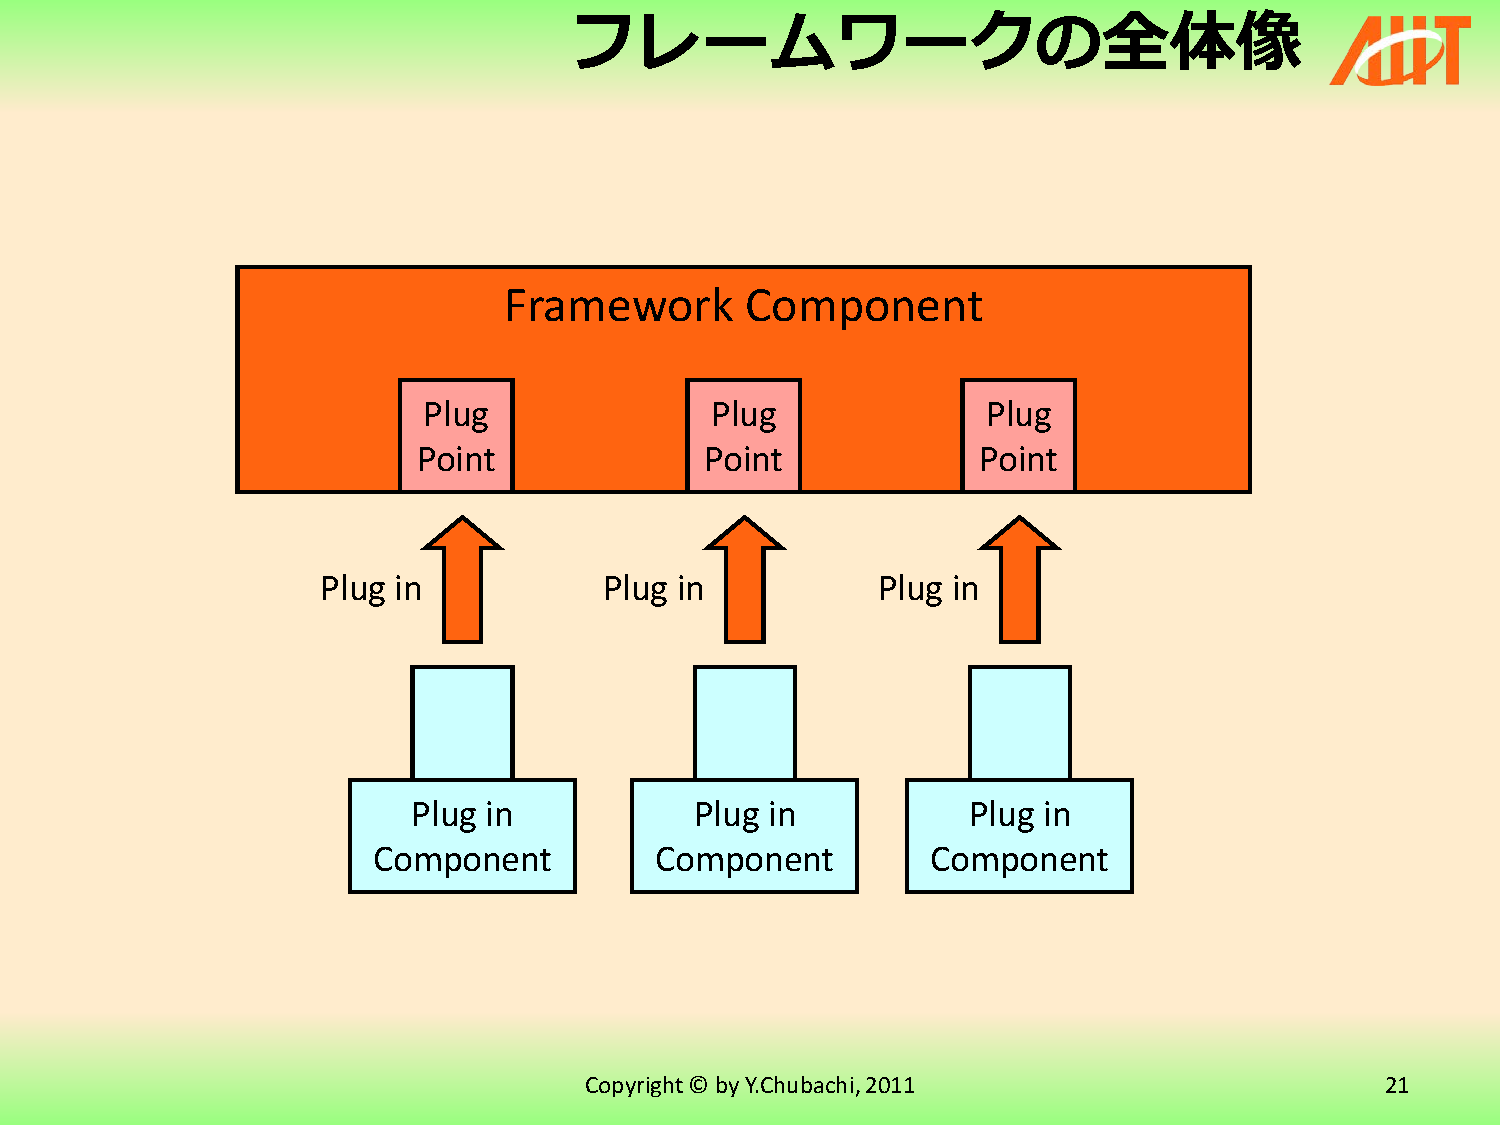
\includegraphics[width=0.8\textwidth, trim=30mm 30mm 35mm
  35mm,clip]{framework.pdf}
  \caption{フレームワークのアーキテクチャ例}\label{fig:framework_architecture}
 \end{center}
\end{figure}

図\ref{fig:framework_architecture}にフレームワークのアーキテクチャを概
念的に示した.

\begin{description}
 \item[コンポーネント(component)] 1つまたはそれ以上のクラスからなる,特
	    定の目的を達成するソフトウェア部品.
 \item[フレームワーク・コンポーネント(framework component)] 再利用性の
	    あるロジックをコンポーネントにしたもので,後述のプラグイン
	    コンポーネントと併用することで,様々なアプリケーションに利
	    用できるソフトウェア部品.
 \item[プラグインコンポーネント(Plug-in Component)] フレームワーク・コ
	    ンポーネントに接続することを前提としたコンポーネントで,必
	    要に応じて作成・カスタマイズできる.
 \item[プラグ・ポイント(Plug point)] コンポーネントをフレームワークに
	    プラグインするために,フレームワークが用意する接続点
\end{description}

\section{フレームワークの作り方}
フレームワークの構築へ向けて

段階を追った学習

もととなるプログラムを段階的に進化させる
方針を立て、プログラミング演習で実装する

アーキテクチャの表現と設計

Java言語の各種のOO機能を活用して、フレームワー
クを構築します

クラス/インタフェイス/メソッド/フィールド/パッ
ケージ・・・

モデル(UML)によりアーキテクチャを表現する

\subsection{リファクタリング・アプローチ}

ボトムアップ・アプローチについて
この授業のスタート地点
 目的の異なる2つのプログラム
フレームワーク構築への道のり
 プログラムの「アーキテクチャ」を捉える
 共通するアーキテクチャを探し出す
 共通化のための方針を立てる
 2つの「上位概念」を考える
 フレームワークを完成させる
リファクタリングとの関連
 このアプローチはリファクタリングの一種でもある

\subsection{ボトムアップ VS トップダウン}

以上説明したボトムアップのアプローチに対して、トップダウンのアプローチというのもある

最初から抽象度の高いアーキテクチャを「モデル」
として設計し、プログラミングで実装する

ボトムアップを採用する理由

初心者にとって学習曲線が緩やかである

実際の開発の現場でも、トップダウンとボトムアッ
プは併用する

\section{MVCパターン}

% $ pdftk フレームワーク開発特論.pdf cat 29 output MVC.pdf
\begin{figure}
 \begin{center}
  %trim option's parameter order: left bottom right top
  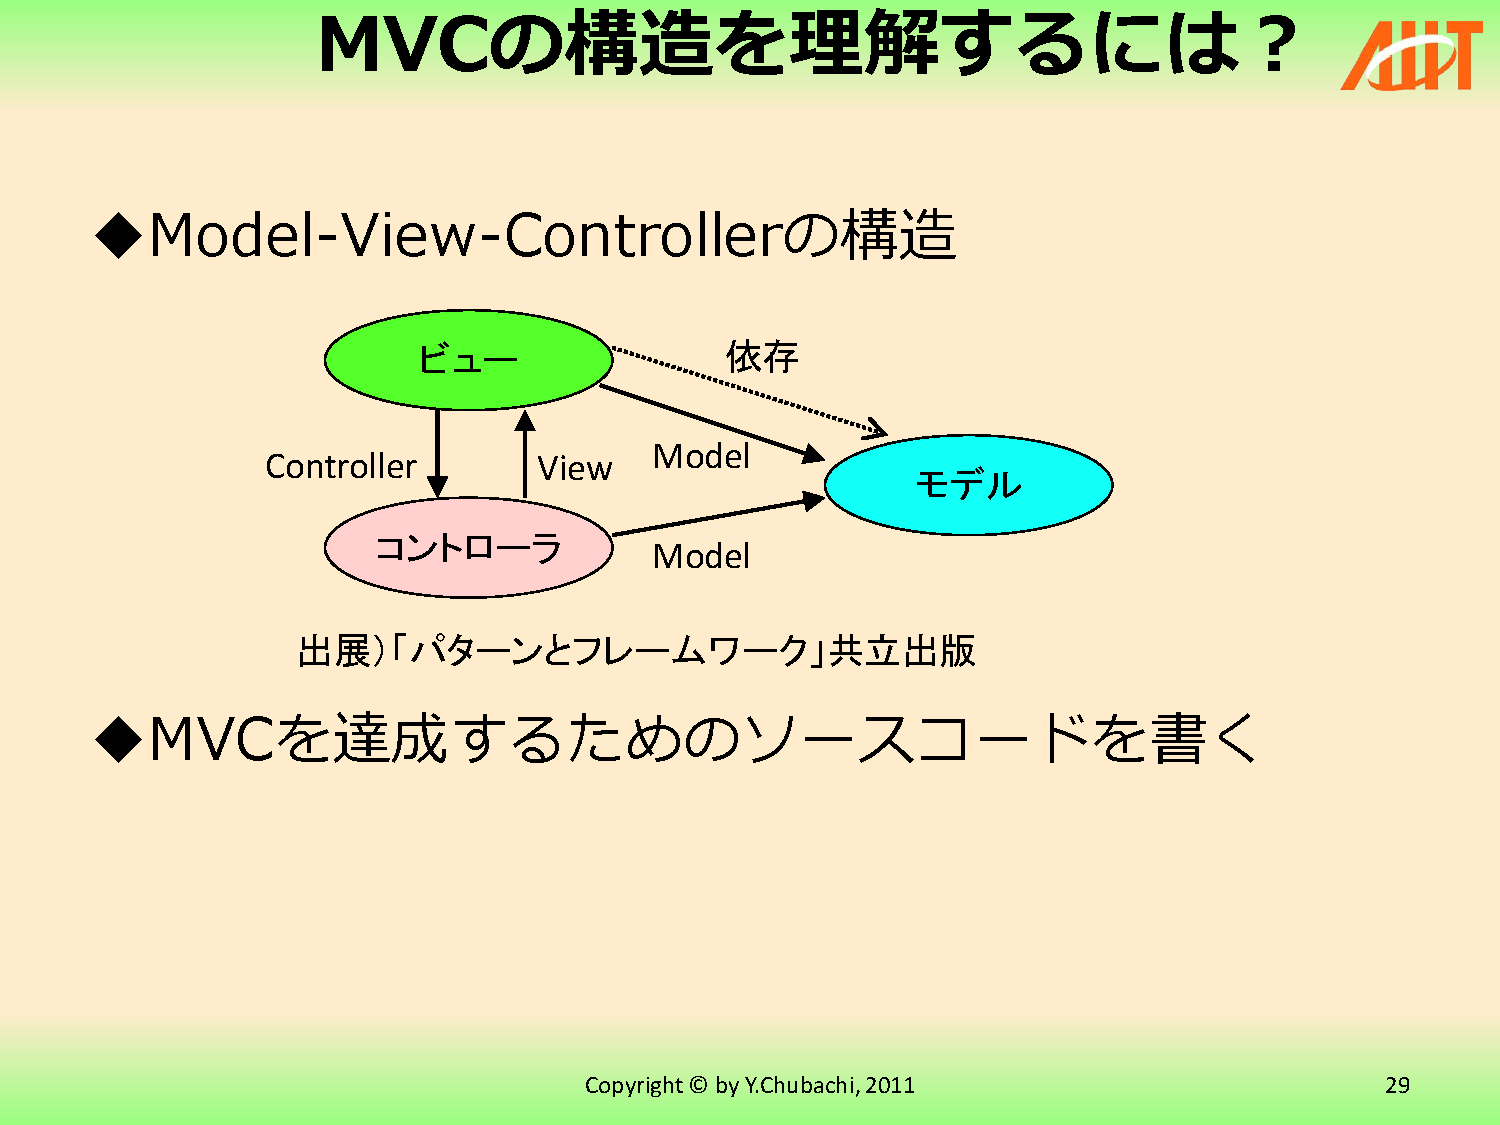
\includegraphics[width=0.8\textwidth, trim=25mm 70mm 60mm 30mm,clip]
   {MVC.pdf}
  \caption{MVC構造(サンプルに合わせて書き直す)}
 \end{center}
\end{figure}

MVC (Model-View-Controller)の重要性
 主にグラフィカルなインタフェースを備えたソフト
ウェアにおいて,広く一般的に利用するフレーム
ワークである
 近年では、Webアプリケーションの構築にも利用す
る
 ただし、伝統的なMVC構造とは異なっている

MVCは何に使われているのか?

GUIを含むアプリケーションの再利用技術

最初の本格的なオブジェクト指向言語である

SmallTalkで採用

MacintoshのUIでも使用

Microsoft Windowsでも採用

Webアプリケーションに適合するよう変化

MVCの構造を理解するには?

Model-View-Controllerの構造

出展)「パターンとフレームワーク」共立出版
MVCを達成するためのソースコードを書く

\subsection{GUIへの適用}
Java言語のSwingクラスライブラリを利用した
MVC構造の実現

自ら作成したMVCの構造を、Swingクラスライブラ
リと組み合わせることで、GUIアプリケーションとし
て完成させる

\subsection{開発環境を活用したプログラミング}
どういう開発環境を使うのか?
• 「Eclipse(エクリプス)」を用いる
• 主にJava言語を用いる開発環境のスタンダード
Eclipseを利用するメリット
• Eclipseはオープンソースの開発環境であり,無料で使うことができる
• コンパイルの自動実行や,文法誤りの発見などの支援を受けることができる
• 大規模なソースコードを管理する機能がある
• 強力なリファクタリング機能
フレームワークとしてのEclipse
• Eclipseそのものがフレームワークを学ぶ教材
• さまざまな機能拡張が可能で,開発者を支援するためのソフトウェア部品が
数多く存在する

\subsection{プログラミング言語は人間が作った}

我々が日常生活で使っている言語(日本語など)を自然言語とするならば,プ
ログラミング言語は人工言語だと言える.

http://merd.sourceforge.net/pixel/language-study/diagram.html

 主要な言語
 詳細な図(150言語以上)

プログラミング言語は人の手で作られた
 Pascalを作った人
 ニクラウス・ヴィルト
 Java言語を作った人
 ジェームズ・ゴスリン
 Perlを作った人
 ラリー・ウォール
 Rubyを作った人
 まつもとゆきひろ
\section{演習問題}
\begin{演習}
身近な次のソフトウェアのIPOはそれぞれなにか?
 ウェブブラウザ
 ワードプロセッサ
 メールリーダ
 データベース
 OS 
\end{演習}

\begin{演習}
「全てのソフトウェアは必ずIPOを備える」は正しいか?
\end{演習}

\begin{演習}
(InputとOutputがない)Processだけのソフトウェアには価値があるか?
\end{演習}

\begin{演習}
IPOフレームワークに基づく「プログラムの価値(=プログラが何を目的として達成する
か)」とは?
\end{演習}

\begin{演習}
 次の???にコメントを書くとしたらどうします
か?
\begin{verbatim}
	double a = 4.56;
	// ???
	int b = (int) (a + 0.5);
	System.out.println(b);
\end{verbatim}
\end{演習}
\section{解答}
\begin{解答}
 視点(領域)の設定や、
粒度によって、答えは異なる
\end{解答}

\chapter{プログラムのアーキテクチャ}

\begin{abstract}
寿限無寿限無五劫の摺り切れ海砂利水魚の水行末雲来末風来末.食う寝る所に住む所藪柑子ブラコウジ.パイポパイポパイポのシューリンガングーリンダイのポンポコピーのポンポコナーの長久命の長助.
\end{abstract}

\section{プログラムの「開始点」}
あなたは,ここ1年以内に,業務で(大学の演習
等を除く)「開始点(mainメソッド)」のある
ソースコードを書いたことがありますか?
ない場合,その理由はなぜですか?

スターティングポイント
 どんなプログラムにも「開始点」がある

開始点の例
 Java言語の場合
 main()メソッド
 C言語の場合
 main()関数
 他の言語の場合は?
 ???

\subsection{Javaのmain()はなぜstaticか?}
仮にMainクラスがあり、コンパイル済みである
とき

 「java Main」コマンドでJVMが起動

 JVMは,クラスのインスタンスを生成しない

 したがって,Mainクラスの通常メソッドは呼び出せ
ない

考えてみよう

 もし,JVM起動時にMainインスタンスを自動生成す
ると?

 プログラマがMainクラスの初期化(コンストラクタへの引
数設定)を制御することができなくなってしまう

– 制御できない=プログラマはとても不自由になる

Javaのmain()でやるべきこと

本来,main()でやるべきこと
 (OSからの引数の受け取り処理)
 中心となる(Main)クラスのインスタンスの生成
 インスタンスの開始メソッド呼び出し
 など

OSの世界とオブジェクト指向の世界の橋渡しをするのがJava言語のmain()の役
割なのだ.

\subsection{Square0: 自乗を計算するプログラム}
\begin{figure}
 \begin{Verbatim}[commandchars=\\\{\},numbers=left,firstnumber=1,stepnumber=1,frame=single,fontsize=\small]
\PY{k+kn}{package}\PY{+w}{ }\PY{n}{square}\PY{o}{;}

\PY{k+kn}{import}\PY{+w}{ }\PY{n+nn}{java.io.BufferedReader}\PY{o}{;}
\PY{k+kn}{import}\PY{+w}{ }\PY{n+nn}{java.io.InputStreamReader}\PY{o}{;}
\PY{k+kn}{import}\PY{+w}{ }\PY{n+nn}{java.io.IOException}\PY{o}{;}

\PY{k+kd}{public}\PY{+w}{ }\PY{k+kd}{class}\PY{+w}{ }\PY{n+nc}{Square}\PY{+w}{ }\PY{o}{\PYZob{}}
\PY{+w}{    }\PY{k+kd}{public}\PY{+w}{ }\PY{k+kd}{static}\PY{+w}{ }\PY{k+kt}{void}\PY{+w}{ }\PY{n+nf}{main}\PY{o}{(}\PY{n}{String}\PY{o}{[}\PY{o}{]}\PY{+w}{ }\PY{n}{args}\PY{o}{)}\PY{+w}{ }\PY{k+kd}{throws}\PY{+w}{ }\PY{n}{IOException}\PY{+w}{ }\PY{o}{\PYZob{}}
\PY{+w}{    }\PY{+w}{    }\PY{n}{System}\PY{o}{.}\PY{n+na}{out}\PY{o}{.}\PY{n+na}{print}\PY{o}{(}\PY{l+s}{"自乗を計算する値を入力してください:"}\PY{o}{)}\PY{o}{;}
\PY{+w}{    }\PY{+w}{    }\PY{n}{BufferedReader}\PY{+w}{ }\PY{n}{reader}\PY{+w}{ }\PY{o}{=}
\PY{+w}{    }\PY{+w}{    }\PY{+w}{    }\PY{k}{new}\PY{+w}{ }\PY{n+nf}{BufferedReader}\PY{o}{(}
\PY{+w}{    }\PY{+w}{    }\PY{+w}{    }\PY{+w}{    }\PY{k}{new}\PY{+w}{ }\PY{n+nf}{InputStreamReader}\PY{o}{(}\PY{n}{System}\PY{o}{.}\PY{n+na}{in}\PY{o}{)}\PY{o}{)}\PY{o}{;}
\PY{+w}{    }\PY{+w}{    }\PY{n}{String}\PY{+w}{ }\PY{n}{valueString}\PY{+w}{ }\PY{o}{=}\PY{+w}{ }\PY{n}{reader}\PY{o}{.}\PY{n+na}{readLine}\PY{o}{(}\PY{o}{)}\PY{o}{;}
\PY{+w}{    }\PY{+w}{    }\PY{k+kt}{double}\PY{+w}{ }\PY{n}{value}\PY{+w}{ }\PY{o}{=}\PY{+w}{ }\PY{n}{Double}\PY{o}{.}\PY{n+na}{parseDouble}\PY{o}{(}\PY{n}{valueString}\PY{o}{)}\PY{o}{;}
\PY{+w}{    }\PY{+w}{    }\PY{n}{System}\PY{o}{.}\PY{n+na}{out}\PY{o}{.}\PY{n+na}{println}\PY{o}{(}\PY{l+s}{"計算結果:"}\PY{+w}{ }\PY{o}{+}\PY{+w}{ }\PY{o}{(}\PY{n}{value}\PY{+w}{ }\PY{o}{*}\PY{+w}{ }\PY{n}{value}\PY{o}{)}\PY{o}{)}\PY{o}{;}
\PY{+w}{    }\PY{o}{\PYZcb{}}
\PY{o}{\PYZcb{}}
\end{Verbatim}

 \caption{Square0: Square.java}\label{fig:Square0:Square}
\end{figure}

最近はあまり見かけないが,一昔前のJava言語の入門書には,プログラムの最
初の例として図\ref{fig:Square0:Square}のようなコードが載っていたもので
ある.入力された値の自乗を計算して表示するためのプログラムだ.

このコードはとても問題のあるコードで,一言で言えば,オブジェクト指向言
語たるJavaらしくないコードなのだ.ある意味,例外的にpublic staticなメソッ
ドになるmain()メソッドにすべての処理が書いてあるという点が問題だ.クラ
スを定義し,そのインスタンスを生成してメソッドを呼ぶ,のがJavaのオブジェ
クト指向というものだろう.

この例を見た,他のプログラミング言語(C言語だのVBだの)を知っている人で
あれば,「では,メソッドでも追加してプログラムを拡張するか」,と考えた
時に,main()の中から作成した他のメソッドが呼べないことに驚くだろう.
staticなメソッドからは,staticなメソッドしか呼べないからだ\marginpar{筆
者は,すべてのメソッドがstaticになっているソートのプログラムを見たこと
がある.C言語の教科書をそのままJava言語に翻訳したものだろう.}.

しかし,前述のとおり,Java言語を初心者に教えようとすると,このコードの
ような例を最初に取り上げるのは致し方がない面がある.だって,すでにたか
がこの程度のプログラムであっても,packageだのimportだのpublicだのclass
だのとおまじないが並ぶ.BufferedReaderやInputStreamReaderといったAPIの
クラス,IOException・・・.誠にJavaは初心者にやさしくない.

これに加えてクラスとインスタンスの理解が必要となる...

1行目はsquareというパッケージ宣言です(正式は?)\marginpar{パッケージ
については・・・を参照.}.

\begin{例題}
 インスタンス生成を用いて書き直せ.ただし,クラスは増やさない.
\end{例題}

\section{クラスとインスタンス}

\subsection{クラスの定義とインスタンスの生成}

\begin{figure}
 \begin{center}
  %trim option's parameter order: left bottom right top
  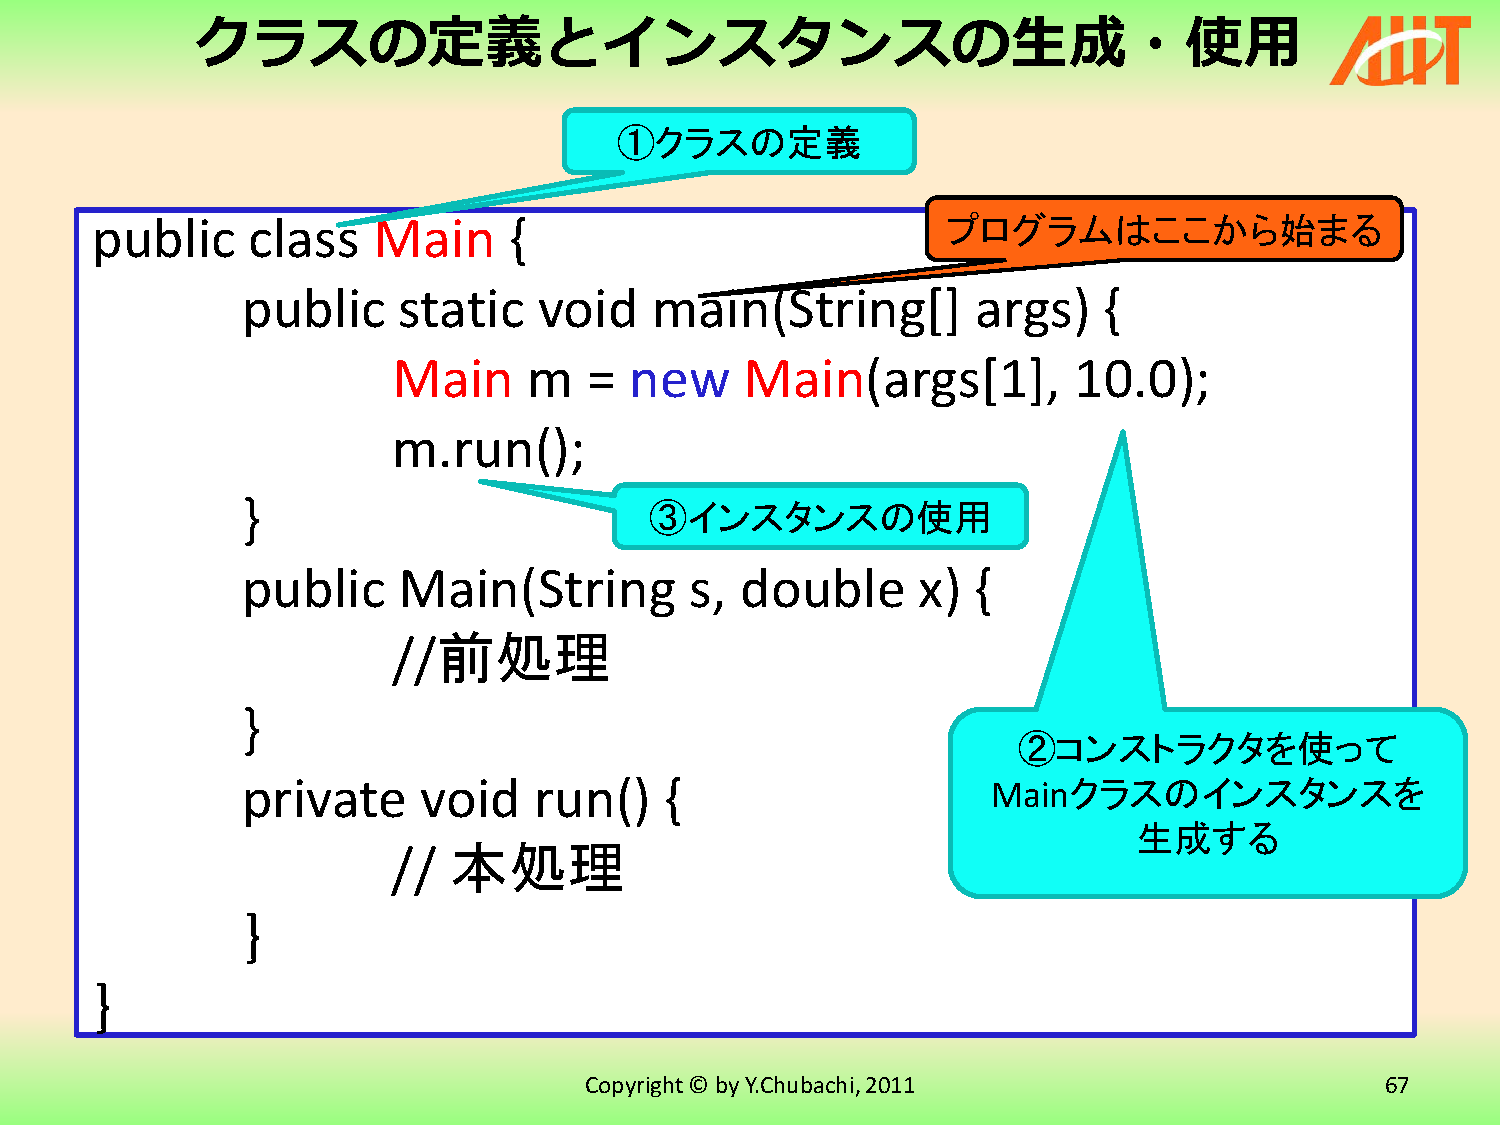
\includegraphics[width=0.8\textwidth, trim=10mm 10mm 5mm 13mm,clip]
   {class_instance.pdf}
  \caption{クラスの定義とインスタンスの生成・使用}
 \end{center}
\end{figure}

Java言語におけるクラスの取り扱い
 クラスを定義する
 インスタンスを生成する
 インスタンスを使用する
 具体的にはメソッド呼び出し
\subsection{Square1: クラスとインスタンス}

\texttt{new}演算子を用い,インスタンスを作成して,メソッドを呼び出す,
オブジェクト指向らしいプログラムにしたのが図\ref{fig:Square1:Square}の
ソースコードである\marginpar{最初に呼び出すメソッドの名前がrun()になっ
ているのは,筆者が最初にプログラミングを学んだBasic言語のrunコマンドが
ある種の原体験として刷り込まれているからなのかもしれない.}.これでやっ
と,落ち着いて先に進める.

\section{IPOパターン}

\begin{figure}
 \begin{Verbatim}[commandchars=\\\{\},numbers=left,firstnumber=1,stepnumber=1,frame=single,fontsize=\small]
\PY{k+kn}{package}\PY{+w}{ }\PY{n}{square}\PY{o}{;}

\PY{k+kn}{import}\PY{+w}{ }\PY{n+nn}{java.io.BufferedReader}\PY{o}{;}
\PY{k+kn}{import}\PY{+w}{ }\PY{n+nn}{java.io.InputStreamReader}\PY{o}{;}

\PY{k+kd}{public}\PY{+w}{ }\PY{k+kd}{class}\PY{+w}{ }\PY{n+nc}{Square}\PY{+w}{ }\PY{o}{\PYZob{}}
\PY{+w}{    }\PY{k+kd}{public}\PY{+w}{ }\PY{k+kd}{static}\PY{+w}{ }\PY{k+kt}{void}\PY{+w}{ }\PY{n+nf}{main}\PY{o}{(}\PY{n}{String}\PY{o}{[}\PY{o}{]}\PY{+w}{ }\PY{n}{args}\PY{o}{)}\PY{+w}{ }\PY{k+kd}{throws}\PY{+w}{ }\PY{n}{Exception}\PY{+w}{ }\PY{o}{\PYZob{}}
\PY{+w}{    }\PY{+w}{    }\PY{n}{Square}\PY{+w}{ }\PY{n}{square}\PY{+w}{ }\PY{o}{=}\PY{+w}{ }\PY{k}{new}\PY{+w}{ }\PY{n}{Square}\PY{o}{(}\PY{o}{)}\PY{o}{;}
\PY{+w}{    }\PY{+w}{    }\PY{n}{square}\PY{o}{.}\PY{n+na}{run}\PY{o}{(}\PY{o}{)}\PY{o}{;}
\PY{+w}{    }\PY{o}{\PYZcb{}}

\PY{+w}{    }\PY{k+kd}{private}\PY{+w}{ }\PY{k+kt}{void}\PY{+w}{ }\PY{n+nf}{run}\PY{o}{(}\PY{o}{)}\PY{+w}{ }\PY{k+kd}{throws}\PY{+w}{ }\PY{n}{Exception}\PY{+w}{ }\PY{o}{\PYZob{}}
\PY{+w}{    }\PY{+w}{    }\PY{n}{System}\PY{o}{.}\PY{n+na}{out}\PY{o}{.}\PY{n+na}{print}\PY{o}{(}\PY{l+s}{"自乗を計算する値を入力してください:"}\PY{o}{)}\PY{o}{;}
\PY{+w}{    }\PY{+w}{    }\PY{n}{BufferedReader}\PY{+w}{ }\PY{n}{reader}\PY{+w}{ }\PY{o}{=}
\PY{+w}{    }\PY{+w}{    }\PY{+w}{    }\PY{k}{new}\PY{+w}{ }\PY{n+nf}{BufferedReader}\PY{o}{(}
\PY{+w}{    }\PY{+w}{    }\PY{+w}{    }\PY{+w}{    }\PY{k}{new}\PY{+w}{ }\PY{n+nf}{InputStreamReader}\PY{o}{(}\PY{n}{System}\PY{o}{.}\PY{n+na}{in}\PY{o}{)}\PY{o}{)}\PY{o}{;}
\PY{+w}{    }\PY{+w}{    }\PY{n}{String}\PY{+w}{ }\PY{n}{valueString}\PY{+w}{ }\PY{o}{=}\PY{+w}{ }\PY{n}{reader}\PY{o}{.}\PY{n+na}{readLine}\PY{o}{(}\PY{o}{)}\PY{o}{;}
\PY{+w}{    }\PY{+w}{    }\PY{k+kt}{double}\PY{+w}{ }\PY{n}{value}\PY{+w}{ }\PY{o}{=}\PY{+w}{ }\PY{n}{Double}\PY{o}{.}\PY{n+na}{parseDouble}\PY{o}{(}\PY{n}{valueString}\PY{o}{)}\PY{o}{;}
\PY{+w}{    }\PY{+w}{    }\PY{n}{System}\PY{o}{.}\PY{n+na}{out}\PY{o}{.}\PY{n+na}{println}\PY{o}{(}\PY{l+s}{"計算結果:"}\PY{+w}{ }\PY{o}{+}\PY{+w}{ }\PY{o}{(}\PY{n}{value}\PY{+w}{ }\PY{o}{*}\PY{+w}{ }\PY{n}{value}\PY{o}{)}\PY{o}{)}\PY{o}{;}
\PY{+w}{    }\PY{o}{\PYZcb{}}
\PY{o}{\PYZcb{}}
\end{Verbatim}

 \caption{Square1: インスタンス生成を用いたSquare.java}\label{fig:Square1:Square}
\end{figure}

最も単純なソフトウェアのアーキテクチャ
 IPO = Input + Process + Output
IPOとは?
 入力処理/中核となる計算処理/出力処理のこと
 株式公開(Initial Public Offering)のことではないです...
ソフトウェアのアーキテクチャの切り口
 IPOをフレームワークとして用いることができる

ソフトウェアはIPOから成り立つ.

\begin{figure}
 \begin{center}
  %trim option's parameter order: left bottom right top
  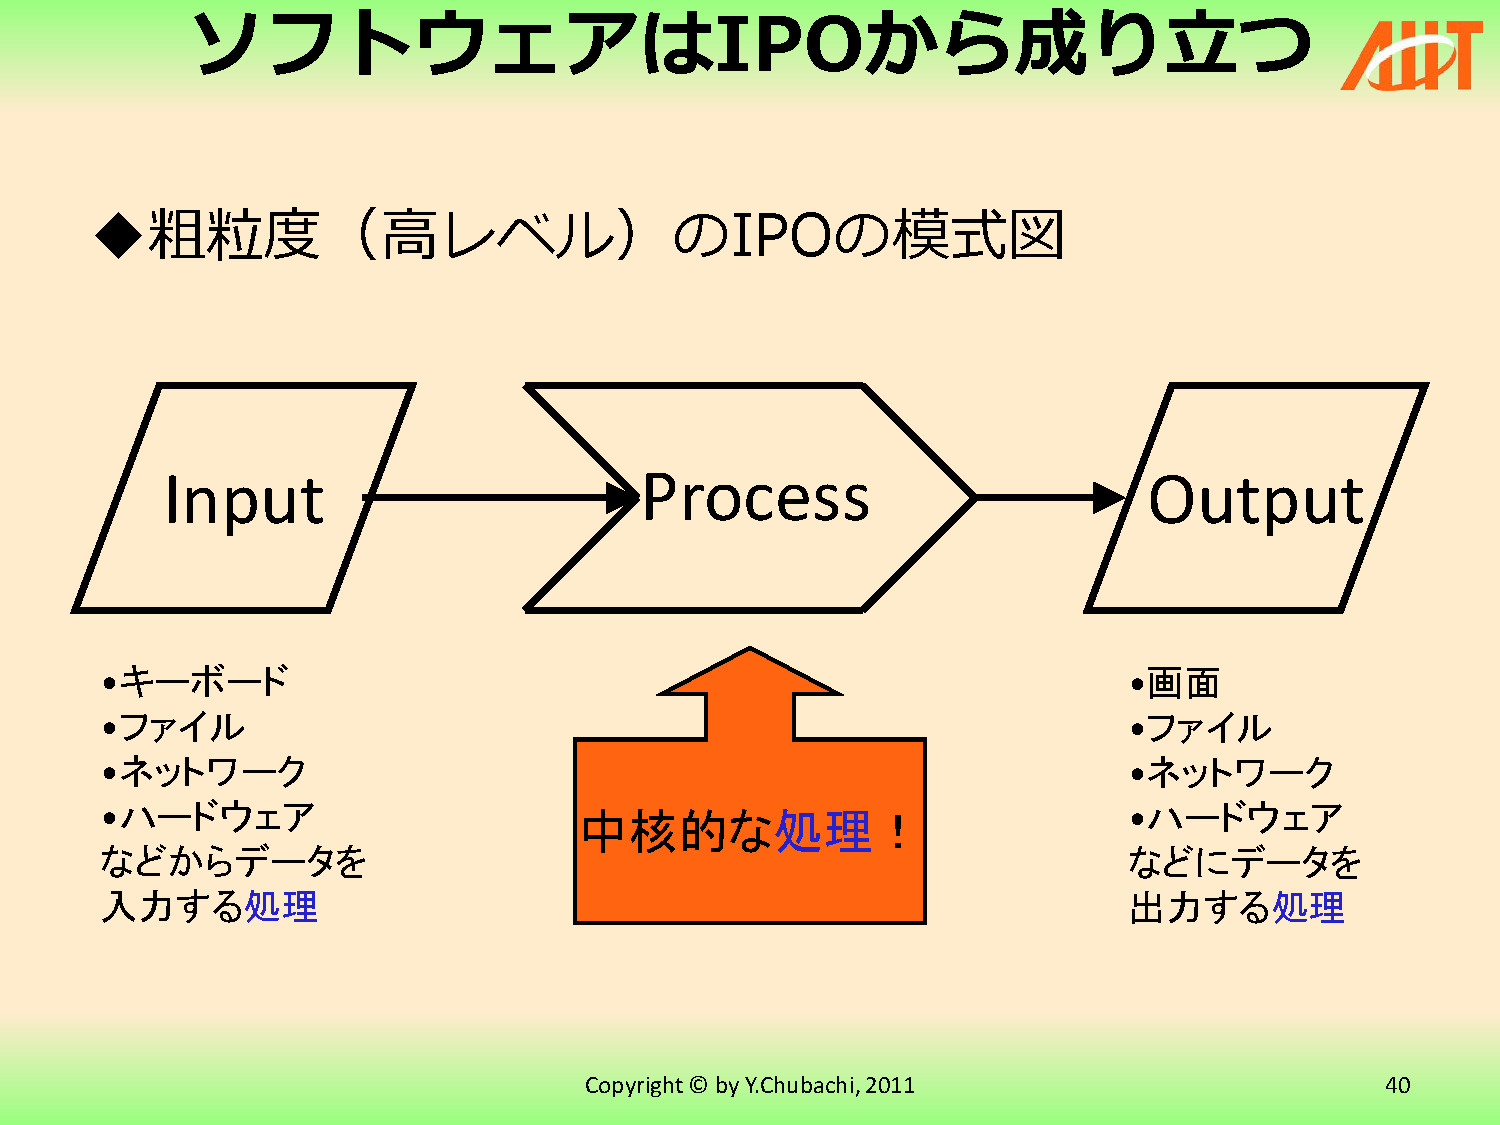
\includegraphics[width=0.8\textwidth, trim=10mm 30mm 10mm 45mm,clip]
   {IPO.pdf}
  \caption{IPOの模式図}
 \end{center}
\end{figure}

大きなIPOはさらに細かいIPO構造を含む.
最終的にはこれ以上細かくできない処理まで行き着く.

\begin{figure}
 \begin{center}
  %trim option's parameter order: left bottom right top
  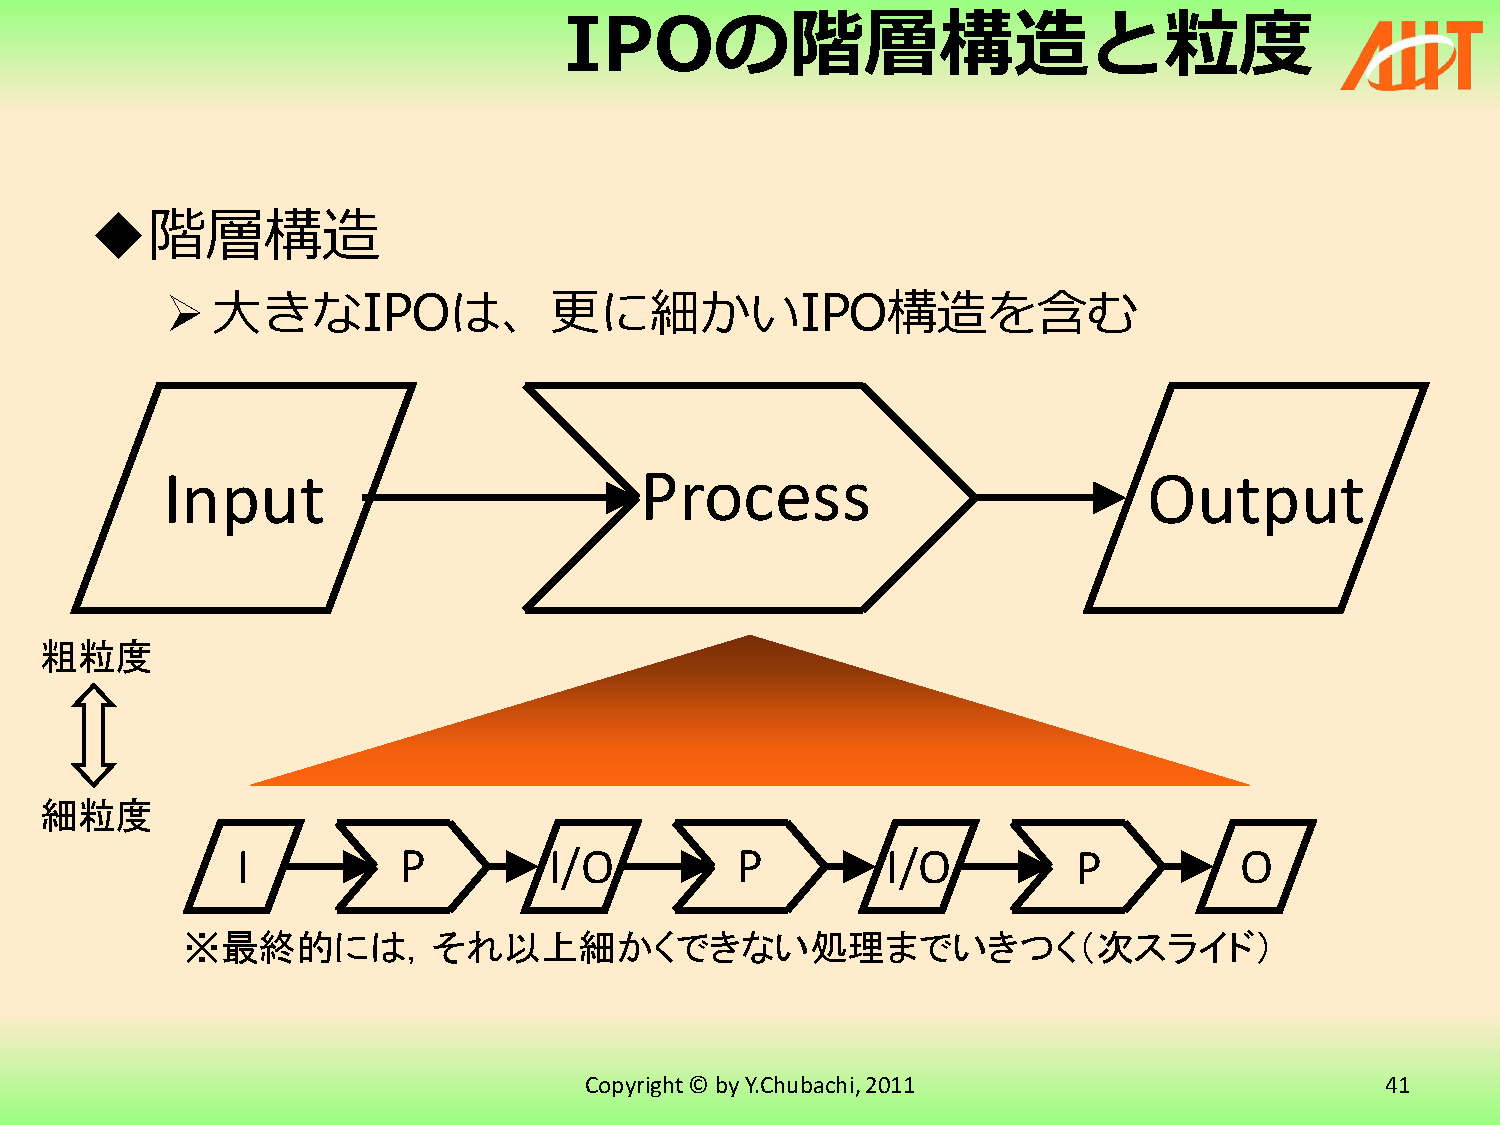
\includegraphics[width=0.8\textwidth, trim=5mm 34mm 10mm 60mm,clip]
   {IPO_tree.pdf}
  \caption{IPOは階層構造になる}
 \end{center}
\end{figure}

最も細かい粒度のIPO

Input
 メモリや
 デバイス
 からデー
タを取り
 込む

Process
 CPUによ
 る演算
 処理

Output
 メモリや
 デバイス
 への
 データの
 送り込み


ここで,次の例題を考えてみよう.

\begin{例題}
 図\ref{fig:Square1:Square}にあるSquareクラスの\texttt{run()}メソッド内
 のコードのうち,入力・処理・出力はそれぞれどこか\marginpar{少し意地の
 悪い問題文の書き方であるが,丁寧に書いてしまっては問題の意味がなくなる
 ので,このような書き方をしておく.}.
\end{例題}

さて,どうやってこの問題をとこうか.

\begin{quotation}
まず目につくのは,14行,20行のSystem.out.println()の箇所ではないだろう
か.このstaticなメソッドは標準出力(通常は画面)に文字列を出力して改行
をする.では,このあたりが「出力」になるのだろうな.

次に「入力」はどこだろうか,と思ってコードを見ると15--17行が標準入力か
ら1行読み込んでいるコードだから,ここらへんがそうか,ふむふむ,となる.

さて,「処理」はというと,残っているのは18-19行なので消去法でここかな….
ここは標準入力から文字列を受け取って,実数型に変換しているコードだから,
処理と言ってもよかろう.

ってでも,このプログラムのそもそもの目的は「自乗を計算」することなんだ
よな.そうすると,自乗を計算している箇所は20行目のvalue * valueだ.そ
うすると,ここも処理なのか.
\end{quotation}

といった(筆者の思惑通りの)思考を巡らせていただけただろうか.いや,巡
らせておいてもらわないとこの後の解説が不要になってしまうから,このよう
に考えた,ということにしておいて強引に説明に進む\marginpar{でも,教室で
この問題を出すと,こういう答えをする学生がほとんどなのだ.まあ,問題文
の書き方に出題者の意図(悪意?)がこめられているからなのであろうが.}.

\section{目的手段展開について}
さて,先ほどあなたは「そもそもの目的は…」と考えたことだろう
\marginpar{くどいようだが,考えたことにして先に進む.}.これがこの例題
を読者に提示している理由と直結している.

\begin{figure}
 \begin{center}
  %trim option's parameter order: left bottom right top
  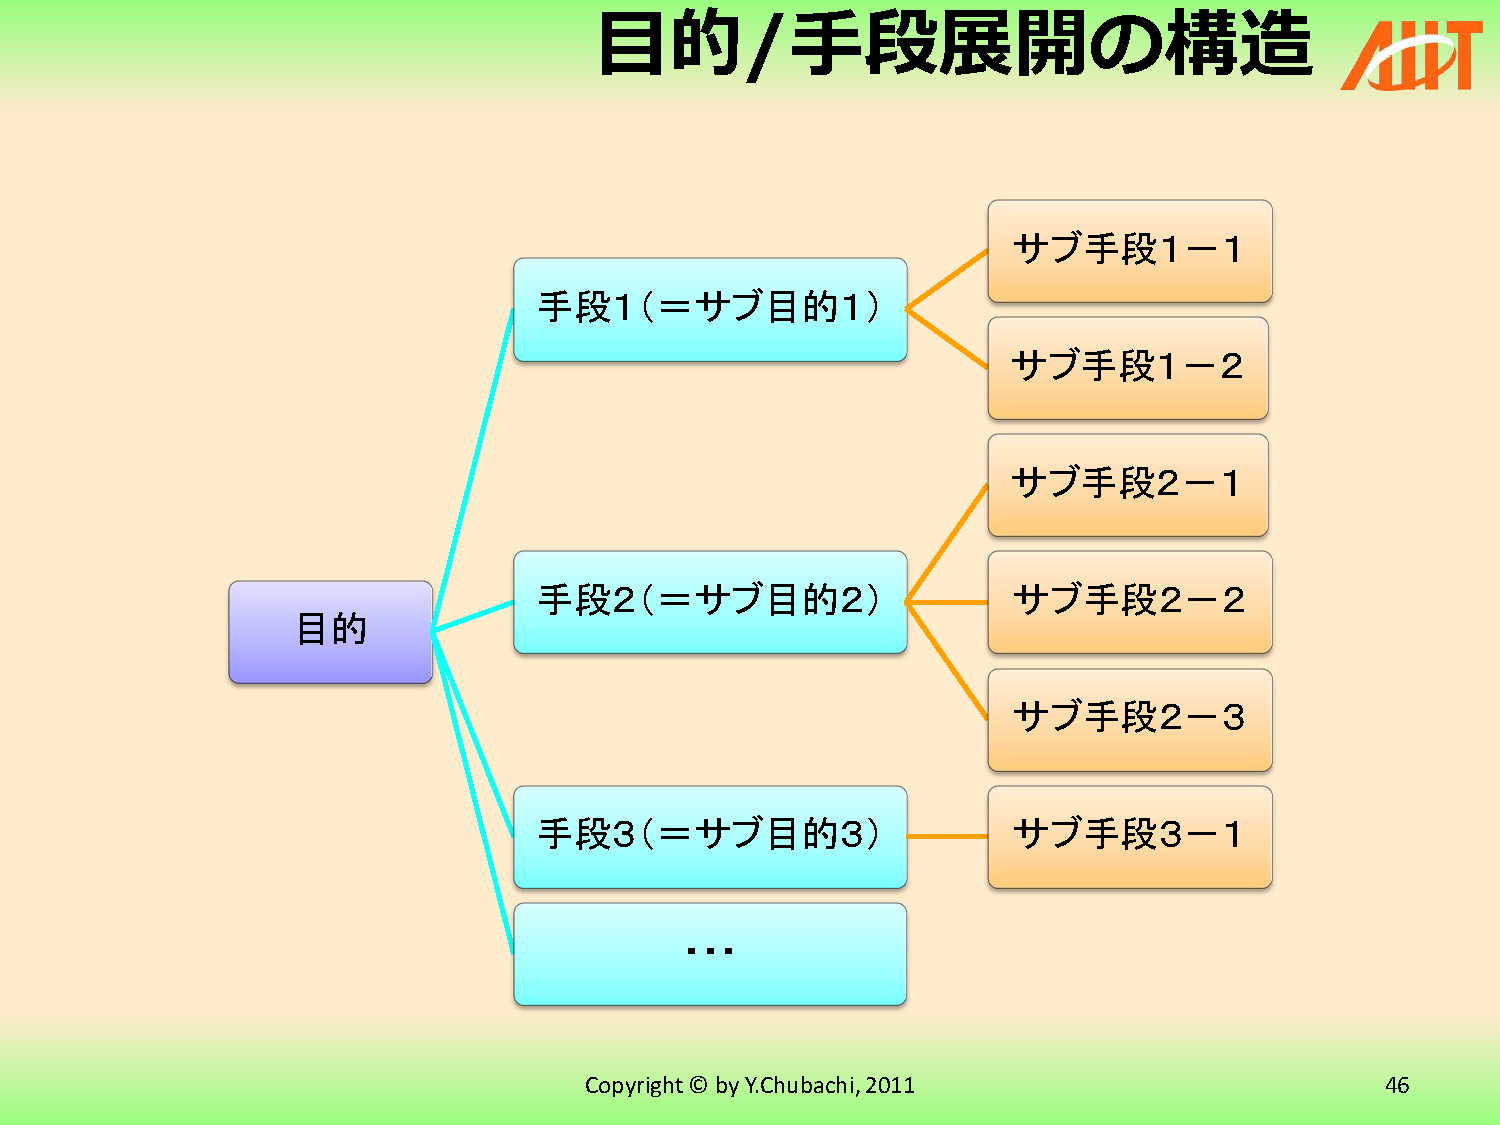
\includegraphics[width=0.8\textwidth, trim=10mm 18mm 20mm 30mm,clip]
   {mokuteki_shudan.pdf}
  \caption{目的手段展開の構造}
 \end{center}
\end{figure}

目的型と手段型のコメント比較

コメントには「目的(何をする・What)」を書
く

「手段(どうする・How)」はコードを読めば分か
る

手段型のコメント
\begin{verbatim}
	// totalをcountで割る
	average = total / count;
\end{verbatim}

目的型のコメント
\begin{verbatim}
	// 平均点を求める
	average = total / count;
\end{verbatim}

\subsection{コメント・ブロック}

コメントによるブロックの作り方.
コメントと空行の組み合わせ.

\begin{verbatim}
private void run() throws Exception {
    // ○○を入力する
    aaa();
    bbb();

    // ○○を計算する
    ccc();

    // ○○を出力する
    ddd();
}
\end{verbatim}

では,実際に,コメント・ブロックを用いてソースコードを分けてみてほしい.

\begin{例題}
ブロックによる構造の整理 

プログラムを編集し,コメントブロックにより
IPOごとに整理しなさい
\end{例題}

 ヒント プロセスとアウトプットを分離するためには,少々工夫が
必要




\subsection{Square2: コメント・ブロック}

\begin{figure}
 \begin{Verbatim}[commandchars=\\\{\},numbers=left,firstnumber=1,stepnumber=1,frame=single,fontsize=\small]
\PY{k+kn}{package}\PY{+w}{ }\PY{n}{square}\PY{o}{;}

\PY{k+kn}{import}\PY{+w}{ }\PY{n+nn}{java.io.BufferedReader}\PY{o}{;}
\PY{k+kn}{import}\PY{+w}{ }\PY{n+nn}{java.io.InputStreamReader}\PY{o}{;}
\PY{k+kn}{import}\PY{+w}{ }\PY{n+nn}{java.io.IOException}\PY{o}{;}

\PY{k+kd}{public}\PY{+w}{ }\PY{k+kd}{class}\PY{+w}{ }\PY{n+nc}{Square}\PY{+w}{ }\PY{o}{\PYZob{}}
\PY{+w}{    }\PY{k+kd}{public}\PY{+w}{ }\PY{k+kd}{static}\PY{+w}{ }\PY{k+kt}{void}\PY{+w}{ }\PY{n+nf}{main}\PY{o}{(}\PY{n}{String}\PY{o}{[}\PY{o}{]}\PY{+w}{ }\PY{n}{args}\PY{o}{)}\PY{+w}{ }\PY{k+kd}{throws}\PY{+w}{ }\PY{n}{IOException}\PY{+w}{ }\PY{o}{\PYZob{}}
\PY{+w}{    }\PY{+w}{    }\PY{n}{Square}\PY{+w}{ }\PY{n}{square}\PY{+w}{ }\PY{o}{=}\PY{+w}{ }\PY{k}{new}\PY{+w}{ }\PY{n}{Square}\PY{o}{(}\PY{o}{)}\PY{o}{;}
\PY{+w}{    }\PY{+w}{    }\PY{n}{square}\PY{o}{.}\PY{n+na}{run}\PY{o}{(}\PY{o}{)}\PY{o}{;}
\PY{+w}{    }\PY{o}{\PYZcb{}}

\PY{+w}{    }\PY{k+kd}{private}\PY{+w}{ }\PY{k+kt}{void}\PY{+w}{ }\PY{n+nf}{run}\PY{o}{(}\PY{o}{)}\PY{+w}{ }\PY{k+kd}{throws}\PY{+w}{ }\PY{n}{IOException}\PY{+w}{ }\PY{o}{\PYZob{}}
\PY{+w}{    }\PY{+w}{    }\PY{c+c1}{//}\PY{+w}{ }\PY{c+c1}{自乗を計算する値を入力する}
\PY{+w}{    }\PY{+w}{    }\PY{k+kt}{double}\PY{+w}{ }\PY{n}{value}\PY{+w}{ }\PY{o}{=}\PY{+w}{ }\PY{n}{input}\PY{o}{(}\PY{o}{)}\PY{o}{;}
\PY{+w}{    }\PY{+w}{    }\PY{c+c1}{//}\PY{+w}{ }\PY{c+c1}{自乗を計算する}
\PY{+w}{    }\PY{+w}{    }\PY{k+kt}{double}\PY{+w}{ }\PY{n}{result}\PY{+w}{ }\PY{o}{=}\PY{+w}{ }\PY{n}{process}\PY{o}{(}\PY{n}{value}\PY{o}{)}\PY{o}{;}
\PY{+w}{    }\PY{+w}{    }\PY{c+c1}{//}\PY{+w}{ }\PY{c+c1}{計算結果を出力する}
\PY{+w}{    }\PY{+w}{    }\PY{n}{output}\PY{o}{(}\PY{n}{result}\PY{o}{)}\PY{o}{;}
\PY{+w}{    }\PY{o}{\PYZcb{}}

\PY{+w}{    }\PY{k+kd}{private}\PY{+w}{ }\PY{k+kt}{double}\PY{+w}{ }\PY{n+nf}{input}\PY{o}{(}\PY{o}{)}\PY{+w}{ }\PY{k+kd}{throws}\PY{+w}{ }\PY{n}{IOException}\PY{+w}{ }\PY{o}{\PYZob{}}
\PY{+w}{    }\PY{+w}{    }\PY{n}{System}\PY{o}{.}\PY{n+na}{out}\PY{o}{.}\PY{n+na}{print}\PY{o}{(}\PY{l+s}{"自乗を計算する値を入力してください:"}\PY{o}{)}\PY{o}{;}
\PY{+w}{    }\PY{+w}{    }\PY{n}{BufferedReader}\PY{+w}{ }\PY{n}{reader}\PY{+w}{ }\PY{o}{=}
\PY{+w}{    }\PY{+w}{    }\PY{+w}{    }\PY{k}{new}\PY{+w}{ }\PY{n+nf}{BufferedReader}\PY{o}{(}
\PY{+w}{    }\PY{+w}{    }\PY{+w}{    }\PY{+w}{    }\PY{k}{new}\PY{+w}{ }\PY{n+nf}{InputStreamReader}\PY{o}{(}\PY{n}{System}\PY{o}{.}\PY{n+na}{in}\PY{o}{)}\PY{o}{)}\PY{o}{;}
\PY{+w}{    }\PY{+w}{    }\PY{n}{String}\PY{+w}{ }\PY{n}{valueString}\PY{+w}{ }\PY{o}{=}\PY{+w}{ }\PY{n}{reader}\PY{o}{.}\PY{n+na}{readLine}\PY{o}{(}\PY{o}{)}\PY{o}{;}
\PY{+w}{    }\PY{+w}{    }\PY{k+kt}{double}\PY{+w}{ }\PY{n}{value}\PY{+w}{ }\PY{o}{=}\PY{+w}{ }\PY{n}{Double}\PY{o}{.}\PY{n+na}{parseDouble}\PY{o}{(}\PY{n}{valueString}\PY{o}{)}\PY{o}{;}
\PY{+w}{    }\PY{+w}{    }\PY{k}{return}\PY{+w}{ }\PY{n}{value}\PY{o}{;}
\PY{+w}{    }\PY{o}{\PYZcb{}}

\PY{+w}{    }\PY{k+kd}{private}\PY{+w}{ }\PY{k+kt}{double}\PY{+w}{ }\PY{n+nf}{process}\PY{o}{(}\PY{k+kt}{double}\PY{+w}{ }\PY{n}{value}\PY{o}{)}\PY{+w}{ }\PY{o}{\PYZob{}}
\PY{+w}{    }\PY{+w}{    }\PY{k+kt}{double}\PY{+w}{ }\PY{n}{result}\PY{+w}{ }\PY{o}{=}\PY{+w}{ }\PY{n}{value}\PY{+w}{ }\PY{o}{*}\PY{+w}{ }\PY{n}{value}\PY{o}{;}
\PY{+w}{    }\PY{+w}{    }\PY{k}{return}\PY{+w}{ }\PY{n}{result}\PY{o}{;}
\PY{+w}{    }\PY{o}{\PYZcb{}}

\PY{+w}{    }\PY{k+kd}{private}\PY{+w}{ }\PY{k+kt}{void}\PY{+w}{ }\PY{n+nf}{output}\PY{o}{(}\PY{k+kt}{double}\PY{+w}{ }\PY{n}{result}\PY{o}{)}\PY{+w}{ }\PY{o}{\PYZob{}}
\PY{+w}{    }\PY{+w}{    }\PY{n}{System}\PY{o}{.}\PY{n+na}{out}\PY{o}{.}\PY{n+na}{println}\PY{o}{(}\PY{l+s}{"計算結果:"}\PY{+w}{ }\PY{o}{+}\PY{+w}{ }\PY{n}{result}\PY{o}{)}\PY{o}{;}
\PY{+w}{    }\PY{o}{\PYZcb{}}
\PY{o}{\PYZcb{}}
\end{Verbatim}

 \caption{Square2: コメント・ブロックで整理したSquareクラス}\label{fig:Square2:Square}
\end{figure}

答えは図\ref{fig:Square2:Square}の通りだ.

最初のコードから変わった点
プログラムの全体構造

 Input-Process-Outputという構造が人間にとって分
かりやすい

 保守性の向上(人に優しいプログラミング)

23行がポイントだ.
人間にとってわかりやすくなった代償として,変数が1つ増えている.

\section{メソッドによる構造化}
コメントブロックの効果と問題
• プログラムのどの部分がIPOを担っているのかが明確
になった
• しかしながら,プログラムの規模が大きくなった場合,
一目で全体構造を捉えることが難しくなる
• コードが長くなるから
一目で分かるメインメソッド
• メイン関数に書いてある記述をメソッドで外部化するこ
とで,プログラムの構造をより見えやすくしよう

IPOをメソッドにする
シンプルでビューティフルなメソッドになる
 プログラムの全体の構造が一目で把握できる

\begin{verbatim}
private void run() throws Exception {
    double input = input();
    double output = process(input);
    output (output);
}
\end{verbatim}

メソッドを利用する目的

同じ処理を複数回利用する

• 一般的なメソッドの利用目的であり,保守性の向上な
どでメリットがある

処理の構造を明確化する

• メソッドには,処理の構造を明確にするという役割が
ある.

• これはすなわち,1度しか呼ばないメソッドであっても,
その作成価値はあるということでもある.

\begin{例題}
 「自乗を計算する」プログラムのメソッド化

 自乗を計算するプログラムのIPOをメソッドにして
みよう
\end{例題}

IPOの各メソッドのシグネチャは次のとおりとする.

\begin{verbatim}
入力: private double input() throws IOException
処理: private double process(double input)
出力: private void output(double output)
\end{verbatim}

\subsection{Square3: IPOをメソッドにする}
IPOをメソッドにしたコードは図\ref{fig:Square3:Square}のとおりになる.

\begin{figure}
 \begin{Verbatim}[commandchars=\\\{\},numbers=left,firstnumber=1,stepnumber=1,frame=single,fontsize=\small]
\PY{k+kn}{package}\PY{+w}{ }\PY{n}{square}\PY{o}{;}

\PY{k+kn}{import}\PY{+w}{ }\PY{n+nn}{java.io.BufferedReader}\PY{o}{;}
\PY{k+kn}{import}\PY{+w}{ }\PY{n+nn}{java.io.InputStreamReader}\PY{o}{;}
\PY{k+kn}{import}\PY{+w}{ }\PY{n+nn}{java.io.IOException}\PY{o}{;}

\PY{k+kd}{public}\PY{+w}{ }\PY{k+kd}{class}\PY{+w}{ }\PY{n+nc}{Square}\PY{+w}{ }\PY{o}{\PYZob{}}
\PY{+w}{    }\PY{k+kd}{public}\PY{+w}{ }\PY{k+kd}{static}\PY{+w}{ }\PY{k+kt}{void}\PY{+w}{ }\PY{n+nf}{main}\PY{o}{(}\PY{n}{String}\PY{o}{[}\PY{o}{]}\PY{+w}{ }\PY{n}{args}\PY{o}{)}\PY{+w}{ }\PY{k+kd}{throws}\PY{+w}{ }\PY{n}{IOException}\PY{+w}{ }\PY{o}{\PYZob{}}
\PY{+w}{    }\PY{+w}{    }\PY{n}{Square}\PY{+w}{ }\PY{n}{square}\PY{+w}{ }\PY{o}{=}\PY{+w}{ }\PY{k}{new}\PY{+w}{ }\PY{n}{Square}\PY{o}{(}\PY{o}{)}\PY{o}{;}
\PY{+w}{    }\PY{+w}{    }\PY{n}{square}\PY{o}{.}\PY{n+na}{run}\PY{o}{(}\PY{o}{)}\PY{o}{;}
\PY{+w}{    }\PY{o}{\PYZcb{}}

\PY{+w}{    }\PY{k+kd}{private}\PY{+w}{ }\PY{k+kt}{void}\PY{+w}{ }\PY{n+nf}{run}\PY{o}{(}\PY{o}{)}\PY{+w}{ }\PY{k+kd}{throws}\PY{+w}{ }\PY{n}{IOException}\PY{+w}{ }\PY{o}{\PYZob{}}
\PY{+w}{    }\PY{+w}{    }\PY{c+c1}{//}\PY{+w}{ }\PY{c+c1}{自乗を計算する値を入力する}
\PY{+w}{    }\PY{+w}{    }\PY{k+kt}{double}\PY{+w}{ }\PY{n}{value}\PY{+w}{ }\PY{o}{=}\PY{+w}{ }\PY{n}{input}\PY{o}{(}\PY{o}{)}\PY{o}{;}
\PY{+w}{    }\PY{+w}{    }\PY{c+c1}{//}\PY{+w}{ }\PY{c+c1}{自乗を計算する}
\PY{+w}{    }\PY{+w}{    }\PY{k+kt}{double}\PY{+w}{ }\PY{n}{result}\PY{+w}{ }\PY{o}{=}\PY{+w}{ }\PY{n}{process}\PY{o}{(}\PY{n}{value}\PY{o}{)}\PY{o}{;}
\PY{+w}{    }\PY{+w}{    }\PY{c+c1}{//}\PY{+w}{ }\PY{c+c1}{計算結果を出力する}
\PY{+w}{    }\PY{+w}{    }\PY{n}{output}\PY{o}{(}\PY{n}{result}\PY{o}{)}\PY{o}{;}
\PY{+w}{    }\PY{o}{\PYZcb{}}

\PY{+w}{    }\PY{k+kd}{private}\PY{+w}{ }\PY{k+kt}{double}\PY{+w}{ }\PY{n+nf}{input}\PY{o}{(}\PY{o}{)}\PY{+w}{ }\PY{k+kd}{throws}\PY{+w}{ }\PY{n}{IOException}\PY{+w}{ }\PY{o}{\PYZob{}}
\PY{+w}{    }\PY{+w}{    }\PY{n}{System}\PY{o}{.}\PY{n+na}{out}\PY{o}{.}\PY{n+na}{print}\PY{o}{(}\PY{l+s}{"自乗を計算する値を入力してください:"}\PY{o}{)}\PY{o}{;}
\PY{+w}{    }\PY{+w}{    }\PY{n}{BufferedReader}\PY{+w}{ }\PY{n}{reader}\PY{+w}{ }\PY{o}{=}
\PY{+w}{    }\PY{+w}{    }\PY{+w}{    }\PY{k}{new}\PY{+w}{ }\PY{n+nf}{BufferedReader}\PY{o}{(}
\PY{+w}{    }\PY{+w}{    }\PY{+w}{    }\PY{+w}{    }\PY{k}{new}\PY{+w}{ }\PY{n+nf}{InputStreamReader}\PY{o}{(}\PY{n}{System}\PY{o}{.}\PY{n+na}{in}\PY{o}{)}\PY{o}{)}\PY{o}{;}
\PY{+w}{    }\PY{+w}{    }\PY{n}{String}\PY{+w}{ }\PY{n}{valueString}\PY{+w}{ }\PY{o}{=}\PY{+w}{ }\PY{n}{reader}\PY{o}{.}\PY{n+na}{readLine}\PY{o}{(}\PY{o}{)}\PY{o}{;}
\PY{+w}{    }\PY{+w}{    }\PY{k+kt}{double}\PY{+w}{ }\PY{n}{value}\PY{+w}{ }\PY{o}{=}\PY{+w}{ }\PY{n}{Double}\PY{o}{.}\PY{n+na}{parseDouble}\PY{o}{(}\PY{n}{valueString}\PY{o}{)}\PY{o}{;}
\PY{+w}{    }\PY{+w}{    }\PY{k}{return}\PY{+w}{ }\PY{n}{value}\PY{o}{;}
\PY{+w}{    }\PY{o}{\PYZcb{}}

\PY{+w}{    }\PY{k+kd}{private}\PY{+w}{ }\PY{k+kt}{double}\PY{+w}{ }\PY{n+nf}{process}\PY{o}{(}\PY{k+kt}{double}\PY{+w}{ }\PY{n}{value}\PY{o}{)}\PY{+w}{ }\PY{o}{\PYZob{}}
\PY{+w}{    }\PY{+w}{    }\PY{k+kt}{double}\PY{+w}{ }\PY{n}{result}\PY{+w}{ }\PY{o}{=}\PY{+w}{ }\PY{n}{value}\PY{+w}{ }\PY{o}{*}\PY{+w}{ }\PY{n}{value}\PY{o}{;}
\PY{+w}{    }\PY{+w}{    }\PY{k}{return}\PY{+w}{ }\PY{n}{result}\PY{o}{;}
\PY{+w}{    }\PY{o}{\PYZcb{}}

\PY{+w}{    }\PY{k+kd}{private}\PY{+w}{ }\PY{k+kt}{void}\PY{+w}{ }\PY{n+nf}{output}\PY{o}{(}\PY{k+kt}{double}\PY{+w}{ }\PY{n}{result}\PY{o}{)}\PY{+w}{ }\PY{o}{\PYZob{}}
\PY{+w}{    }\PY{+w}{    }\PY{n}{System}\PY{o}{.}\PY{n+na}{out}\PY{o}{.}\PY{n+na}{println}\PY{o}{(}\PY{l+s}{"計算結果:"}\PY{+w}{ }\PY{o}{+}\PY{+w}{ }\PY{n}{result}\PY{o}{)}\PY{o}{;}
\PY{+w}{    }\PY{o}{\PYZcb{}}
\PY{o}{\PYZcb{}}
\end{Verbatim}

 \caption{Square3: メソッドで構造化したSquareクラス}\label{fig:Square3:Square}
\end{figure}

\begin{figure}
 \begin{center}
  %trim option's parameter order: left bottom right top
  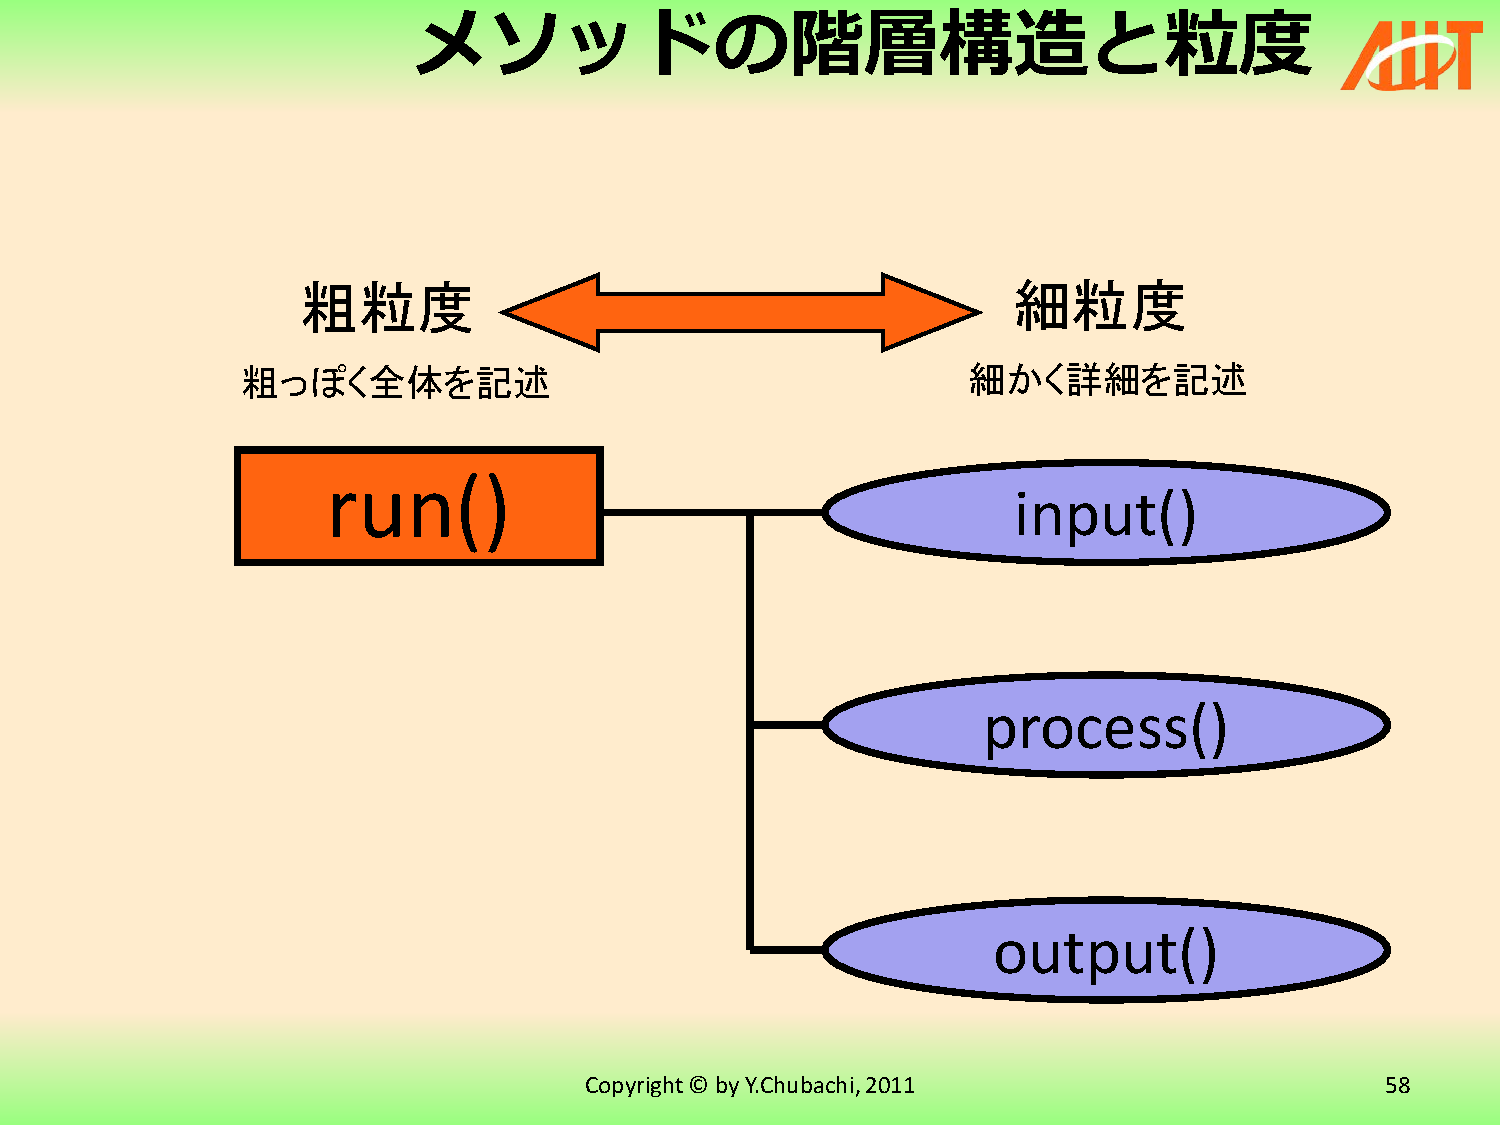
\includegraphics[width=0.8\textwidth, trim=33mm 18mm 15mm 35mm,clip]
   {run.pdf}
  \caption{メソッドの階層構造}
 \end{center}
\end{figure}

\subsection{メソッドのシグネチャ}

メソッドのシグネチャと戻り値の型
メソッドのシグネチャ(signature)とは?
 あるメソッドと他のメソッドを区別するためのもの
シグネチャの構成要素(一般的なもの)
Java言語では、
 メソッド名
他に限定子・例外も
シグネチャに含めます
 引数の数と型
 戻り値の型・・・(Java言語では考慮されない)
シグネチャの例
 public static void main(String[] args)
 メソッド名:
 引数の数と型:
 戻り値の型:
main
Stringの配列が1つ
void

メソッドの「宣言」と「実装」

メソッドの宣言とは?

 メソッドの「シグネチャ」を定義すること

メソッドの実装とは?

 メソッドの宣言に基づき,メソッドの実際の振る舞
いを記述すること

「宣言」と「実装」を分離して考える理由

 他のメソッドから,あるメソッドを呼び出す場合,
呼び出し側はそのメソッドの「宣言」に適合してい
ればよい

 「実装」については考えなくてもよい
Java言語の宣言と実装
通常,Java言語では,メソッドの「宣言」と
「実装」を同時に取り扱う

\begin{figure}
 \begin{center}
  %trim option's parameter order: left bottom right top
  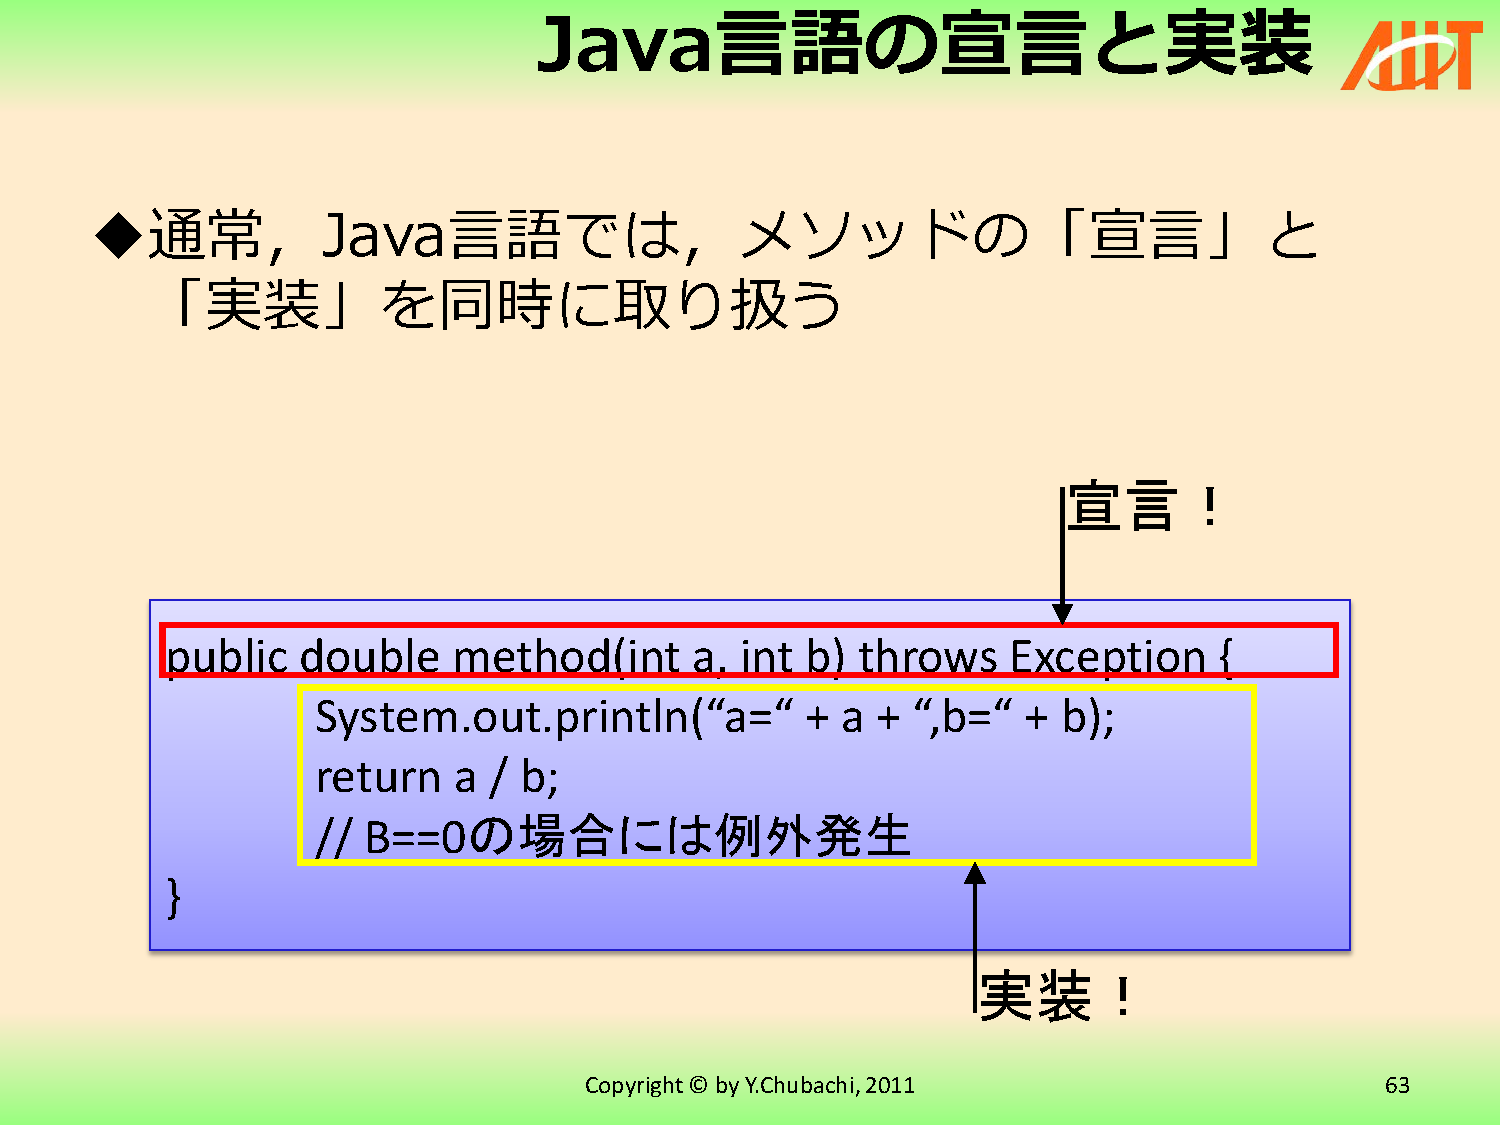
\includegraphics[width=0.8\textwidth, trim=15mm 15mm 15mm 75mm,clip]
   {signature.pdf}
  \caption{Java言語の宣言と実装}
 \end{center}
\end{figure}

\newpage
\section{演習問題}

\begin{演習}
 図\ref{fig:Division1:Division}のプログラムをコメント・ブロックにより入
 力・処理・出力の構造を明確にせよ.
\end{演習}

\begin{figure}
 \begin{Verbatim}[commandchars=\\\{\},numbers=left,firstnumber=1,stepnumber=1,frame=single,fontsize=\small]
\PY{k+kn}{package}\PY{+w}{ }\PY{n}{division}\PY{o}{;}

\PY{k+kn}{import}\PY{+w}{ }\PY{n+nn}{java.io.BufferedReader}\PY{o}{;}
\PY{k+kn}{import}\PY{+w}{ }\PY{n+nn}{java.io.InputStreamReader}\PY{o}{;}

\PY{k+kd}{public}\PY{+w}{ }\PY{k+kd}{class}\PY{+w}{ }\PY{n+nc}{Division}\PY{+w}{ }\PY{o}{\PYZob{}}
\PY{+w}{    }\PY{k+kd}{public}\PY{+w}{ }\PY{k+kd}{static}\PY{+w}{ }\PY{k+kt}{void}\PY{+w}{ }\PY{n+nf}{main}\PY{o}{(}\PY{n}{String}\PY{o}{[}\PY{o}{]}\PY{+w}{ }\PY{n}{args}\PY{o}{)}\PY{+w}{ }\PY{k+kd}{throws}\PY{+w}{ }\PY{n}{Exception}\PY{+w}{ }\PY{o}{\PYZob{}}
\PY{+w}{    }\PY{+w}{    }\PY{n}{Division}\PY{+w}{ }\PY{n}{division}\PY{+w}{ }\PY{o}{=}\PY{+w}{ }\PY{k}{new}\PY{+w}{ }\PY{n}{Division}\PY{o}{(}\PY{o}{)}\PY{o}{;}
\PY{+w}{    }\PY{+w}{    }\PY{n}{division}\PY{o}{.}\PY{n+na}{run}\PY{o}{(}\PY{o}{)}\PY{o}{;}
\PY{+w}{    }\PY{o}{\PYZcb{}}
\PY{+w}{    }
\PY{+w}{    }\PY{k+kd}{private}\PY{+w}{ }\PY{k+kt}{void}\PY{+w}{ }\PY{n+nf}{run}\PY{o}{(}\PY{o}{)}\PY{+w}{ }\PY{k+kd}{throws}\PY{+w}{ }\PY{n}{Exception}\PY{+w}{ }\PY{o}{\PYZob{}}
\PY{+w}{    }\PY{+w}{    }\PY{n}{BufferedReader}\PY{+w}{ }\PY{n}{reader}\PY{+w}{ }\PY{o}{=}
\PY{+w}{    }\PY{+w}{    }\PY{+w}{    }\PY{k}{new}\PY{+w}{ }\PY{n+nf}{BufferedReader}\PY{o}{(}\PY{k}{new}\PY{+w}{ }\PY{n}{InputStreamReader}\PY{o}{(}\PY{n}{System}\PY{o}{.}\PY{n+na}{in}\PY{o}{)}\PY{o}{)}\PY{o}{;}
\PY{+w}{    }\PY{+w}{    }\PY{n}{System}\PY{o}{.}\PY{n+na}{out}\PY{o}{.}\PY{n+na}{print}\PY{o}{(}\PY{l+s}{"割られる数を入力してください:"}\PY{o}{)}\PY{o}{;}
\PY{+w}{    }\PY{+w}{    }\PY{n}{String}\PY{+w}{ }\PY{n}{dividendString}\PY{+w}{ }\PY{o}{=}\PY{+w}{ }\PY{n}{reader}\PY{o}{.}\PY{n+na}{readLine}\PY{o}{(}\PY{o}{)}\PY{o}{;}
\PY{+w}{    }\PY{+w}{    }\PY{k+kt}{int}\PY{+w}{ }\PY{n}{dividend}\PY{+w}{ }\PY{o}{=}\PY{+w}{ }\PY{n}{Integer}\PY{o}{.}\PY{n+na}{parseInt}\PY{o}{(}\PY{n}{dividendString}\PY{o}{)}\PY{o}{;}
\PY{+w}{    }\PY{+w}{    }\PY{n}{System}\PY{o}{.}\PY{n+na}{out}\PY{o}{.}\PY{n+na}{print}\PY{o}{(}\PY{l+s}{"割る数を入力してください:"}\PY{o}{)}\PY{o}{;}
\PY{+w}{    }\PY{+w}{    }\PY{n}{String}\PY{+w}{ }\PY{n}{divisorString}\PY{+w}{ }\PY{o}{=}\PY{+w}{ }\PY{n}{reader}\PY{o}{.}\PY{n+na}{readLine}\PY{o}{(}\PY{o}{)}\PY{o}{;}
\PY{+w}{    }\PY{+w}{    }\PY{k+kt}{int}\PY{+w}{ }\PY{n}{divisor}\PY{+w}{ }\PY{o}{=}\PY{+w}{ }\PY{n}{Integer}\PY{o}{.}\PY{n+na}{parseInt}\PY{o}{(}\PY{n}{divisorString}\PY{o}{)}\PY{o}{;}
\PY{+w}{    }\PY{+w}{    }\PY{n}{System}\PY{o}{.}\PY{n+na}{out}\PY{o}{.}\PY{n+na}{print}\PY{o}{(}\PY{l+s}{"商は"}\PY{+w}{ }\PY{o}{+}\PY{+w}{ }\PY{n}{dividend}\PY{+w}{ }\PY{o}{/}\PY{+w}{ }\PY{n}{divisor}
\PY{+w}{    }\PY{+w}{    }\PY{+w}{    }\PY{+w}{    }\PY{o}{+}\PY{+w}{ }\PY{l+s}{"で余は"}\PY{+w}{ }\PY{o}{+}\PY{+w}{ }\PY{n}{dividend}\PY{+w}{ }\PY{o}{\PYZpc{}}\PY{+w}{ }\PY{n}{divisor}\PY{+w}{ }\PY{o}{+}\PY{+w}{ }\PY{l+s}{"です"}\PY{o}{)}\PY{o}{;}
\PY{+w}{    }\PY{o}{\PYZcb{}}
\PY{o}{\PYZcb{}}
\end{Verbatim}

 \caption{Division1: 割り算を計算するプログラム}\label{fig:Division1:Division}
\end{figure}


\chapter{入出力クラス}

\begin{abstract}
 入力と出力をクラスに...
\end{abstract}

\section{Division2: 割り算の入出力値にクラスを導入}

\begin{figure}
 \begin{Verbatim}[commandchars=\\\{\},numbers=left,firstnumber=1,stepnumber=1,frame=single,fontsize=\small]
\PY{k+kn}{package}\PY{+w}{ }\PY{n}{division}\PY{o}{;}

\PY{k+kn}{import}\PY{+w}{ }\PY{n+nn}{java.io.BufferedReader}\PY{o}{;}
\PY{k+kn}{import}\PY{+w}{ }\PY{n+nn}{java.io.InputStreamReader}\PY{o}{;}

\PY{k+kd}{public}\PY{+w}{ }\PY{k+kd}{class}\PY{+w}{ }\PY{n+nc}{Division}\PY{+w}{ }\PY{o}{\PYZob{}}
\PY{+w}{    }\PY{k+kd}{public}\PY{+w}{ }\PY{k+kd}{static}\PY{+w}{ }\PY{k+kt}{void}\PY{+w}{ }\PY{n+nf}{main}\PY{o}{(}\PY{n}{String}\PY{o}{[}\PY{o}{]}\PY{+w}{ }\PY{n}{args}\PY{o}{)}\PY{+w}{ }\PY{k+kd}{throws}\PY{+w}{ }\PY{n}{Exception}\PY{+w}{ }\PY{o}{\PYZob{}}
\PY{+w}{    }\PY{+w}{    }\PY{n}{Division}\PY{+w}{ }\PY{n}{division}\PY{+w}{ }\PY{o}{=}\PY{+w}{ }\PY{k}{new}\PY{+w}{ }\PY{n}{Division}\PY{o}{(}\PY{o}{)}\PY{o}{;}
\PY{+w}{    }\PY{+w}{    }\PY{n}{division}\PY{o}{.}\PY{n+na}{run}\PY{o}{(}\PY{o}{)}\PY{o}{;}
\PY{+w}{    }\PY{o}{\PYZcb{}}
\PY{+w}{    }
\PY{+w}{    }\PY{k+kd}{private}\PY{+w}{ }\PY{k+kt}{void}\PY{+w}{ }\PY{n+nf}{run}\PY{o}{(}\PY{o}{)}\PY{+w}{ }\PY{k+kd}{throws}\PY{+w}{ }\PY{n}{Exception}\PY{+w}{ }\PY{o}{\PYZob{}}
\PY{+w}{    }\PY{+w}{    }\PY{c+c1}{//}\PY{+w}{ }\PY{c+c1}{割られる数と割る数を読み込む}
\PY{+w}{    }\PY{+w}{    }\PY{n}{BufferedReader}\PY{+w}{ }\PY{n}{reader}\PY{+w}{ }\PY{o}{=}
\PY{+w}{    }\PY{+w}{    }\PY{+w}{    }\PY{k}{new}\PY{+w}{ }\PY{n+nf}{BufferedReader}\PY{o}{(}\PY{k}{new}\PY{+w}{ }\PY{n}{InputStreamReader}\PY{o}{(}\PY{n}{System}\PY{o}{.}\PY{n+na}{in}\PY{o}{)}\PY{o}{)}\PY{o}{;}
\PY{+w}{    }\PY{+w}{    }\PY{n}{System}\PY{o}{.}\PY{n+na}{out}\PY{o}{.}\PY{n+na}{print}\PY{o}{(}\PY{l+s}{"割られる数を入力してください:"}\PY{o}{)}\PY{o}{;}
\PY{+w}{    }\PY{+w}{    }\PY{n}{String}\PY{+w}{ }\PY{n}{dividendString}\PY{+w}{ }\PY{o}{=}\PY{+w}{ }\PY{n}{reader}\PY{o}{.}\PY{n+na}{readLine}\PY{o}{(}\PY{o}{)}\PY{o}{;}
\PY{+w}{    }\PY{+w}{    }\PY{k+kt}{int}\PY{+w}{ }\PY{n}{dividend}\PY{+w}{ }\PY{o}{=}\PY{+w}{ }\PY{n}{Integer}\PY{o}{.}\PY{n+na}{parseInt}\PY{o}{(}\PY{n}{dividendString}\PY{o}{)}\PY{o}{;}
\PY{+w}{    }\PY{+w}{    }\PY{n}{System}\PY{o}{.}\PY{n+na}{out}\PY{o}{.}\PY{n+na}{print}\PY{o}{(}\PY{l+s}{"割る数を入力してください:"}\PY{o}{)}\PY{o}{;}
\PY{+w}{    }\PY{+w}{    }\PY{n}{String}\PY{+w}{ }\PY{n}{divisorString}\PY{+w}{ }\PY{o}{=}\PY{+w}{ }\PY{n}{reader}\PY{o}{.}\PY{n+na}{readLine}\PY{o}{(}\PY{o}{)}\PY{o}{;}
\PY{+w}{    }\PY{+w}{    }\PY{k+kt}{int}\PY{+w}{ }\PY{n}{divisor}\PY{+w}{ }\PY{o}{=}\PY{+w}{ }\PY{n}{Integer}\PY{o}{.}\PY{n+na}{parseInt}\PY{o}{(}\PY{n}{divisorString}\PY{o}{)}\PY{o}{;}
\PY{+w}{    }\PY{+w}{    }
\PY{+w}{    }\PY{+w}{    }\PY{c+c1}{//}\PY{+w}{ }\PY{c+c1}{商と余を計算する}
\PY{+w}{    }\PY{+w}{    }\PY{k+kt}{int}\PY{+w}{ }\PY{n}{quotient}\PY{+w}{ }\PY{o}{=}\PY{+w}{ }\PY{n}{dividend}\PY{+w}{ }\PY{o}{/}\PY{+w}{ }\PY{n}{divisor}\PY{o}{;}
\PY{+w}{    }\PY{+w}{    }\PY{k+kt}{int}\PY{+w}{ }\PY{n}{remainder}\PY{+w}{ }\PY{o}{=}\PY{+w}{ }\PY{n}{dividend}\PY{+w}{ }\PY{o}{\PYZpc{}}\PY{+w}{ }\PY{n}{divisor}\PY{o}{;}

\PY{+w}{    }\PY{+w}{    }\PY{c+c1}{//}\PY{+w}{ }\PY{c+c1}{割り算の結果を表示する}
\PY{+w}{    }\PY{+w}{    }\PY{n}{System}\PY{o}{.}\PY{n+na}{out}\PY{o}{.}\PY{n+na}{print}\PY{o}{(}\PY{l+s}{"商は"}\PY{+w}{ }\PY{o}{+}\PY{+w}{ }\PY{n}{quotient}\PY{+w}{ }\PY{o}{+}\PY{+w}{ }\PY{l+s}{"で余は"}\PY{+w}{ }\PY{o}{+}\PY{+w}{ }\PY{n}{remainder}\PY{+w}{ }\PY{o}{+}\PY{+w}{ }\PY{l+s}{"です"}\PY{o}{)}\PY{o}{;}
\PY{+w}{    }\PY{o}{\PYZcb{}}
\PY{o}{\PYZcb{}}
\end{Verbatim}

 \caption{Division2: コメント・ブロックで整理したDivisionクラス}\label{fig:Division2:Division}
\end{figure}

メソッドによる構造化は便利な手段であるが,図
\ref{fig:Division2:Division}のコードをメソッドで整理しようとするとちょっ
とした工夫が必要だ\marginpar{これは前の演習の答え.}.

\begin{例題}
 図\ref{fig:Division2:Division} のコードをメソッドで整理せよ.
\end{例題}

演習?で取り上げた「割り算を計算する」プログラムは,

• このプログラムは,割られる数と割る数を入力に取り,
商と余を返す

• 即ち,入力値が2つ,出力値も2つである

\section{Javaのメソッドの文法上の制約}

Java言語のメソッドの制限

 Java言語のメソッドは,複数の値を入力として受け取ることはできるが,複数の
値を出力することができない\marginpar{他のプログラミング言語(LispやPerl
など)は,複数の出力値を返すメソッド(関数)を作成できるものもある.リストやハッシュ表として.}


• この問題を解決するには,どうしたらよいだろうか?

Java言語のメソッドは,次の構造である

 出力値=メソッド(入力値1,入力値2,...入力値n)

割り算を計算するプログラムには,出力値が2つあ
る

 自乗を計算するプログラムの場合と同様の方法で入出力を
メソッドにすることはできない

 Eclipseのリファクタリング機能も使えない

\section{複数の値を束ねるクラス}

この問題を「クラス」を導入することで解決しよう

 注意)


複数の値を束ねる手段としてのクラス
ここでは,Javaのクラスが持つ多くの性質のう
ち,「複数の値を束ねる」側面を使ってみよう

入出力クラスを使ったメソッド

次のようなコードが可能になるため,複数の入
力値・出力値をメソッドに引き渡すことができ
る

\begin{verbatim}
	入力クラス input;
	出力クラス output;
	output = 処理(input)
\end{verbatim}

なお,別な方法として,参照渡しを使って次のよう
にすることもできるが,まずはシンプルな方法を採
用する

\begin{verbatim}
	入力クラス input = new 入力クラス();
	出力クラス output = new 出力クラス();
	処理(input, output)
\end{verbatim}


なお,メソッドはまだ導入しなくて良い.

「割る数と割られる数」は図\ref{fig:Division3:DividendAndDivisor}のクラスで表そう.
\begin{figure}
 \begin{Verbatim}[commandchars=\\\{\},numbers=left,firstnumber=1,stepnumber=1,frame=single,fontsize=\small]
\PY{k+kn}{package}\PY{+w}{ }\PY{n}{division}\PY{o}{;}

\PY{k+kd}{class}\PY{+w}{ }\PY{n+nc}{DividendAndDivisor}\PY{+w}{ }\PY{o}{\PYZob{}}
\PY{+w}{    }\PY{k+kt}{int}\PY{+w}{ }\PY{n}{dividend}\PY{o}{;}
\PY{+w}{    }\PY{k+kt}{int}\PY{+w}{ }\PY{n}{divisor}\PY{o}{;}
\PY{o}{\PYZcb{}}
\end{Verbatim}

 \caption{Division3: 割る数と割られる数クラス}\label{fig:Division3:DividendAndDivisor}
\end{figure}


「商と余」は図\ref{fig:Division3:QuotientAndRemainder}のクラスを用いる.
\begin{figure}
 \begin{Verbatim}[commandchars=\\\{\},numbers=left,firstnumber=1,stepnumber=1,frame=single,fontsize=\small]
\PY{k+kn}{package}\PY{+w}{ }\PY{n}{division}\PY{o}{;}

\PY{k+kd}{class}\PY{+w}{ }\PY{n+nc}{QuotientAndRemainder}\PY{+w}{ }\PY{o}{\PYZob{}}
\PY{+w}{    }\PY{k+kt}{int}\PY{+w}{ }\PY{n}{quotient}\PY{o}{;}
\PY{+w}{    }\PY{k+kt}{int}\PY{+w}{ }\PY{n}{remainder}\PY{o}{;}
\PY{o}{\PYZcb{}}
\end{Verbatim}

 \caption{Division3: 商と余クラス}\label{fig:Division3:QuotientAndRemainder}
\end{figure}

2つのクラスを導入したコードは図\ref{fig:Division3:Division}のとおりだ.
14行と25行がインスタンスを生成している部分である.

\begin{figure}
 \begin{Verbatim}[commandchars=\\\{\},numbers=left,firstnumber=1,stepnumber=1,frame=single,fontsize=\small]
\PY{k+kn}{package}\PY{+w}{ }\PY{n}{division}\PY{o}{;}

\PY{k+kn}{import}\PY{+w}{ }\PY{n+nn}{java.io.BufferedReader}\PY{o}{;}
\PY{k+kn}{import}\PY{+w}{ }\PY{n+nn}{java.io.InputStreamReader}\PY{o}{;}

\PY{k+kd}{public}\PY{+w}{ }\PY{k+kd}{class}\PY{+w}{ }\PY{n+nc}{Division}\PY{+w}{ }\PY{o}{\PYZob{}}
\PY{+w}{    }\PY{k+kd}{public}\PY{+w}{ }\PY{k+kd}{static}\PY{+w}{ }\PY{k+kt}{void}\PY{+w}{ }\PY{n+nf}{main}\PY{o}{(}\PY{n}{String}\PY{o}{[}\PY{o}{]}\PY{+w}{ }\PY{n}{args}\PY{o}{)}\PY{+w}{ }\PY{k+kd}{throws}\PY{+w}{ }\PY{n}{Exception}\PY{+w}{ }\PY{o}{\PYZob{}}
\PY{+w}{    }\PY{+w}{    }\PY{n}{Division}\PY{+w}{ }\PY{n}{division}\PY{+w}{ }\PY{o}{=}\PY{+w}{ }\PY{k}{new}\PY{+w}{ }\PY{n}{Division}\PY{o}{(}\PY{o}{)}\PY{o}{;}
\PY{+w}{    }\PY{+w}{    }\PY{n}{division}\PY{o}{.}\PY{n+na}{run}\PY{o}{(}\PY{o}{)}\PY{o}{;}
\PY{+w}{    }\PY{o}{\PYZcb{}}
\PY{+w}{    }
\PY{+w}{    }\PY{k+kd}{private}\PY{+w}{ }\PY{k+kt}{void}\PY{+w}{ }\PY{n+nf}{run}\PY{o}{(}\PY{o}{)}\PY{+w}{ }\PY{k+kd}{throws}\PY{+w}{ }\PY{n}{Exception}\PY{+w}{ }\PY{o}{\PYZob{}}
\PY{+w}{    }\PY{+w}{    }\PY{c+c1}{//}\PY{+w}{ }\PY{c+c1}{割られる数と割る数を読み込む}
\PY{+w}{    }\PY{+w}{    }\PY{n}{DividendAndDivisor}\PY{+w}{ }\PY{n}{input}\PY{+w}{ }\PY{o}{=}\PY{+w}{ }\PY{k}{new}\PY{+w}{ }\PY{n}{DividendAndDivisor}\PY{o}{(}\PY{o}{)}\PY{o}{;}
\PY{+w}{    }\PY{+w}{    }\PY{n}{BufferedReader}\PY{+w}{ }\PY{n}{reader}\PY{+w}{ }\PY{o}{=}
\PY{+w}{    }\PY{+w}{    }\PY{+w}{    }\PY{k}{new}\PY{+w}{ }\PY{n+nf}{BufferedReader}\PY{o}{(}\PY{k}{new}\PY{+w}{ }\PY{n}{InputStreamReader}\PY{o}{(}\PY{n}{System}\PY{o}{.}\PY{n+na}{in}\PY{o}{)}\PY{o}{)}\PY{o}{;}
\PY{+w}{    }\PY{+w}{    }\PY{n}{System}\PY{o}{.}\PY{n+na}{out}\PY{o}{.}\PY{n+na}{print}\PY{o}{(}\PY{l+s}{"割られる数を入力してください:"}\PY{o}{)}\PY{o}{;}
\PY{+w}{    }\PY{+w}{    }\PY{n}{String}\PY{+w}{ }\PY{n}{dividendString}\PY{+w}{ }\PY{o}{=}\PY{+w}{ }\PY{n}{reader}\PY{o}{.}\PY{n+na}{readLine}\PY{o}{(}\PY{o}{)}\PY{o}{;}
\PY{+w}{    }\PY{+w}{    }\PY{n}{input}\PY{o}{.}\PY{n+na}{dividend}\PY{+w}{ }\PY{o}{=}\PY{+w}{ }\PY{n}{Integer}\PY{o}{.}\PY{n+na}{parseInt}\PY{o}{(}\PY{n}{dividendString}\PY{o}{)}\PY{o}{;}
\PY{+w}{    }\PY{+w}{    }\PY{n}{System}\PY{o}{.}\PY{n+na}{out}\PY{o}{.}\PY{n+na}{print}\PY{o}{(}\PY{l+s}{"割る数を入力してください:"}\PY{o}{)}\PY{o}{;}
\PY{+w}{    }\PY{+w}{    }\PY{n}{String}\PY{+w}{ }\PY{n}{divisorString}\PY{+w}{ }\PY{o}{=}\PY{+w}{ }\PY{n}{reader}\PY{o}{.}\PY{n+na}{readLine}\PY{o}{(}\PY{o}{)}\PY{o}{;}
\PY{+w}{    }\PY{+w}{    }\PY{n}{input}\PY{o}{.}\PY{n+na}{divisor}\PY{+w}{ }\PY{o}{=}\PY{+w}{ }\PY{n}{Integer}\PY{o}{.}\PY{n+na}{parseInt}\PY{o}{(}\PY{n}{divisorString}\PY{o}{)}\PY{o}{;}
\PY{+w}{    }\PY{+w}{    }
\PY{+w}{    }\PY{+w}{    }\PY{c+c1}{//}\PY{+w}{ }\PY{c+c1}{商と余を計算する}
\PY{+w}{    }\PY{+w}{    }\PY{n}{QuotientAndRemainder}\PY{+w}{ }\PY{n}{output}\PY{+w}{ }\PY{o}{=}\PY{+w}{ }\PY{k}{new}\PY{+w}{ }\PY{n}{QuotientAndRemainder}\PY{o}{(}\PY{o}{)}\PY{o}{;}
\PY{+w}{    }\PY{+w}{    }\PY{n}{output}\PY{o}{.}\PY{n+na}{quotient}\PY{+w}{ }\PY{o}{=}\PY{+w}{ }\PY{n}{input}\PY{o}{.}\PY{n+na}{dividend}\PY{+w}{ }\PY{o}{/}\PY{+w}{ }\PY{n}{input}\PY{o}{.}\PY{n+na}{divisor}\PY{o}{;}
\PY{+w}{    }\PY{+w}{    }\PY{n}{output}\PY{o}{.}\PY{n+na}{remainder}\PY{+w}{ }\PY{o}{=}\PY{+w}{ }\PY{n}{input}\PY{o}{.}\PY{n+na}{dividend}\PY{+w}{ }\PY{o}{\PYZpc{}}\PY{+w}{ }\PY{n}{input}\PY{o}{.}\PY{n+na}{divisor}\PY{o}{;}

\PY{+w}{    }\PY{+w}{    }\PY{c+c1}{//}\PY{+w}{ }\PY{c+c1}{割り算の結果を表示する}
\PY{+w}{    }\PY{+w}{    }\PY{n}{System}\PY{o}{.}\PY{n+na}{out}\PY{o}{.}\PY{n+na}{print}\PY{o}{(}\PY{l+s}{"商は"}\PY{+w}{ }\PY{o}{+}\PY{+w}{ }\PY{n}{output}\PY{o}{.}\PY{n+na}{quotient}
\PY{+w}{    }\PY{+w}{    }\PY{+w}{    }\PY{+w}{    }\PY{o}{+}\PY{+w}{ }\PY{l+s}{"で余は"}\PY{+w}{ }\PY{o}{+}\PY{+w}{ }\PY{n}{output}\PY{o}{.}\PY{n+na}{remainder}\PY{+w}{ }\PY{o}{+}\PY{+w}{ }\PY{l+s}{"です"}\PY{o}{)}\PY{o}{;}
\PY{+w}{    }\PY{o}{\PYZcb{}}
\PY{o}{\PYZcb{}}
\end{Verbatim}

 \caption{Division3: 入出力をクラスに変更したDivision}\label{fig:Division3:Division}
\end{figure}

\section{Division3: メソッド化}
\begin{例題}
 メソッドを導入せよ.
\end{例題}

新しい\texttt{run()}は次のとおりになるだろう.

\begin{verbatim}
	private void run() throws Exception {
	    DividendAndDivisor input = input();
	    QuotientAndRemainder output = process(input);
	    output (output);
	}
\end{verbatim}

入出力値クラスはそのまま使う.

図\ref{fig:Division4:Division}になる.

\begin{figure}
 \begin{Verbatim}[commandchars=\\\{\},numbers=left,firstnumber=1,stepnumber=1,frame=single,fontsize=\small]
\PY{k+kn}{package}\PY{+w}{ }\PY{n}{division}\PY{o}{;}

\PY{k+kn}{import}\PY{+w}{ }\PY{n+nn}{java.io.BufferedReader}\PY{o}{;}
\PY{k+kn}{import}\PY{+w}{ }\PY{n+nn}{java.io.IOException}\PY{o}{;}
\PY{k+kn}{import}\PY{+w}{ }\PY{n+nn}{java.io.InputStreamReader}\PY{o}{;}

\PY{k+kd}{public}\PY{+w}{ }\PY{k+kd}{class}\PY{+w}{ }\PY{n+nc}{Division}\PY{+w}{ }\PY{o}{\PYZob{}}
\PY{+w}{    }\PY{k+kd}{public}\PY{+w}{ }\PY{k+kd}{static}\PY{+w}{ }\PY{k+kt}{void}\PY{+w}{ }\PY{n+nf}{main}\PY{o}{(}\PY{n}{String}\PY{o}{[}\PY{o}{]}\PY{+w}{ }\PY{n}{args}\PY{o}{)}\PY{+w}{ }\PY{k+kd}{throws}\PY{+w}{ }\PY{n}{Exception}\PY{+w}{ }\PY{o}{\PYZob{}}
\PY{+w}{    }\PY{+w}{    }\PY{n}{Division}\PY{+w}{ }\PY{n}{division}\PY{+w}{ }\PY{o}{=}\PY{+w}{ }\PY{k}{new}\PY{+w}{ }\PY{n}{Division}\PY{o}{(}\PY{o}{)}\PY{o}{;}
\PY{+w}{    }\PY{+w}{    }\PY{n}{division}\PY{o}{.}\PY{n+na}{run}\PY{o}{(}\PY{o}{)}\PY{o}{;}
\PY{+w}{    }\PY{o}{\PYZcb{}}
\PY{+w}{    }
\PY{+w}{    }\PY{k+kd}{private}\PY{+w}{ }\PY{k+kt}{void}\PY{+w}{ }\PY{n+nf}{run}\PY{o}{(}\PY{o}{)}\PY{+w}{ }\PY{k+kd}{throws}\PY{+w}{ }\PY{n}{Exception}\PY{+w}{ }\PY{o}{\PYZob{}}
\PY{+w}{    }\PY{+w}{    }\PY{c+c1}{//}\PY{+w}{ }\PY{c+c1}{割られる数と割る数を読み込む}
\PY{+w}{    }\PY{+w}{    }\PY{n}{DividendAndDivisor}\PY{+w}{ }\PY{n}{input}\PY{+w}{ }\PY{o}{=}\PY{+w}{ }\PY{n}{input}\PY{o}{(}\PY{o}{)}\PY{o}{;}
\PY{+w}{    }\PY{+w}{    }\PY{c+c1}{//}\PY{+w}{ }\PY{c+c1}{商と余を計算する}
\PY{+w}{    }\PY{+w}{    }\PY{n}{QuotientAndRemainder}\PY{+w}{ }\PY{n}{output}\PY{+w}{ }\PY{o}{=}\PY{+w}{ }\PY{n}{process}\PY{o}{(}\PY{n}{input}\PY{o}{)}\PY{o}{;}
\PY{+w}{    }\PY{+w}{    }\PY{c+c1}{//}\PY{+w}{ }\PY{c+c1}{割り算の結果を表示する}
\PY{+w}{    }\PY{+w}{    }\PY{n}{output}\PY{o}{(}\PY{n}{output}\PY{o}{)}\PY{o}{;}
\PY{+w}{    }\PY{o}{\PYZcb{}}

\PY{+w}{    }\PY{k+kd}{private}\PY{+w}{ }\PY{n}{DividendAndDivisor}\PY{+w}{ }\PY{n+nf}{input}\PY{o}{(}\PY{o}{)}\PY{+w}{ }\PY{k+kd}{throws}\PY{+w}{ }\PY{n}{IOException}\PY{+w}{ }\PY{o}{\PYZob{}}
\PY{+w}{    }\PY{+w}{    }\PY{n}{DividendAndDivisor}\PY{+w}{ }\PY{n}{input}\PY{+w}{ }\PY{o}{=}\PY{+w}{ }\PY{k}{new}\PY{+w}{ }\PY{n}{DividendAndDivisor}\PY{o}{(}\PY{o}{)}\PY{o}{;}
\PY{+w}{    }\PY{+w}{    }\PY{n}{BufferedReader}\PY{+w}{ }\PY{n}{reader}\PY{+w}{ }\PY{o}{=}
\PY{+w}{    }\PY{+w}{    }\PY{+w}{    }\PY{k}{new}\PY{+w}{ }\PY{n+nf}{BufferedReader}\PY{o}{(}\PY{k}{new}\PY{+w}{ }\PY{n}{InputStreamReader}\PY{o}{(}\PY{n}{System}\PY{o}{.}\PY{n+na}{in}\PY{o}{)}\PY{o}{)}\PY{o}{;}
\PY{+w}{    }\PY{+w}{    }\PY{n}{System}\PY{o}{.}\PY{n+na}{out}\PY{o}{.}\PY{n+na}{print}\PY{o}{(}\PY{l+s}{"割られる数を入力してください:"}\PY{o}{)}\PY{o}{;}
\PY{+w}{    }\PY{+w}{    }\PY{n}{String}\PY{+w}{ }\PY{n}{dividendString}\PY{+w}{ }\PY{o}{=}\PY{+w}{ }\PY{n}{reader}\PY{o}{.}\PY{n+na}{readLine}\PY{o}{(}\PY{o}{)}\PY{o}{;}
\PY{+w}{    }\PY{+w}{    }\PY{n}{input}\PY{o}{.}\PY{n+na}{dividend}\PY{+w}{ }\PY{o}{=}\PY{+w}{ }\PY{n}{Integer}\PY{o}{.}\PY{n+na}{parseInt}\PY{o}{(}\PY{n}{dividendString}\PY{o}{)}\PY{o}{;}
\PY{+w}{    }\PY{+w}{    }\PY{n}{System}\PY{o}{.}\PY{n+na}{out}\PY{o}{.}\PY{n+na}{print}\PY{o}{(}\PY{l+s}{"割る数を入力してください:"}\PY{o}{)}\PY{o}{;}
\PY{+w}{    }\PY{+w}{    }\PY{n}{String}\PY{+w}{ }\PY{n}{divisorString}\PY{+w}{ }\PY{o}{=}\PY{+w}{ }\PY{n}{reader}\PY{o}{.}\PY{n+na}{readLine}\PY{o}{(}\PY{o}{)}\PY{o}{;}
\PY{+w}{    }\PY{+w}{    }\PY{n}{input}\PY{o}{.}\PY{n+na}{divisor}\PY{+w}{ }\PY{o}{=}\PY{+w}{ }\PY{n}{Integer}\PY{o}{.}\PY{n+na}{parseInt}\PY{o}{(}\PY{n}{divisorString}\PY{o}{)}\PY{o}{;}
\PY{+w}{    }\PY{+w}{    }\PY{k}{return}\PY{+w}{ }\PY{n}{input}\PY{o}{;}
\PY{+w}{    }\PY{o}{\PYZcb{}}

\PY{+w}{    }\PY{k+kd}{private}\PY{+w}{ }\PY{n}{QuotientAndRemainder}\PY{+w}{ }\PY{n+nf}{process}\PY{o}{(}\PY{n}{DividendAndDivisor}\PY{+w}{ }\PY{n}{input}\PY{o}{)}\PY{+w}{ }\PY{o}{\PYZob{}}
\PY{+w}{    }\PY{+w}{    }\PY{n}{QuotientAndRemainder}\PY{+w}{ }\PY{n}{output}\PY{+w}{ }\PY{o}{=}\PY{+w}{ }\PY{k}{new}\PY{+w}{ }\PY{n}{QuotientAndRemainder}\PY{o}{(}\PY{o}{)}\PY{o}{;}
\PY{+w}{    }\PY{+w}{    }\PY{n}{output}\PY{o}{.}\PY{n+na}{quotient}\PY{+w}{ }\PY{o}{=}\PY{+w}{ }\PY{n}{input}\PY{o}{.}\PY{n+na}{dividend}\PY{+w}{ }\PY{o}{/}\PY{+w}{ }\PY{n}{input}\PY{o}{.}\PY{n+na}{divisor}\PY{o}{;}
\PY{+w}{    }\PY{+w}{    }\PY{n}{output}\PY{o}{.}\PY{n+na}{remainder}\PY{+w}{ }\PY{o}{=}\PY{+w}{ }\PY{n}{input}\PY{o}{.}\PY{n+na}{dividend}\PY{+w}{ }\PY{o}{\PYZpc{}}\PY{+w}{ }\PY{n}{input}\PY{o}{.}\PY{n+na}{divisor}\PY{o}{;}
\PY{+w}{    }\PY{+w}{    }\PY{k}{return}\PY{+w}{ }\PY{n}{output}\PY{o}{;}
\PY{+w}{    }\PY{o}{\PYZcb{}}

\PY{+w}{    }\PY{k+kd}{private}\PY{+w}{ }\PY{k+kt}{void}\PY{+w}{ }\PY{n+nf}{output}\PY{o}{(}\PY{n}{QuotientAndRemainder}\PY{+w}{ }\PY{n}{output}\PY{o}{)}\PY{+w}{ }\PY{o}{\PYZob{}}
\PY{+w}{    }\PY{+w}{    }\PY{n}{System}\PY{o}{.}\PY{n+na}{out}\PY{o}{.}\PY{n+na}{print}\PY{o}{(}\PY{l+s}{"商は"}\PY{+w}{ }\PY{o}{+}\PY{+w}{ }\PY{n}{output}\PY{o}{.}\PY{n+na}{quotient}\PY{+w}{ }\PY{o}{+}\PY{+w}{ }\PY{l+s}{"で余は"}\PY{+w}{ }\PY{o}{+}\PY{+w}{ }\PY{n}{output}\PY{o}{.}\PY{n+na}{remainder}\PY{+w}{ }\PY{o}{+}\PY{+w}{ }\PY{l+s}{"です"}\PY{o}{)}\PY{o}{;}
\PY{+w}{    }\PY{o}{\PYZcb{}}
\PY{o}{\PYZcb{}}
\end{Verbatim}

 \caption{Division4: メソッドによる構造化をしたDivision}\label{fig:Division4:Division}
\end{figure}

\newpage

\section{演習}
\begin{演習}
 図\ref{fig:Square4:Square}頁のコードの入力・出力の値をクラスにせよ.
\end{演習}

カプセル化.図\ref{fig:Square4:ValueToBeSquared},図\ref{fig:Square4:SquaredValue}参照.

\begin{figure}
 \begin{Verbatim}[commandchars=\\\{\},numbers=left,firstnumber=1,stepnumber=1,frame=single,fontsize=\small]
\PY{k+kn}{package}\PY{+w}{ }\PY{n}{square}\PY{o}{;}

\PY{k+kd}{class}\PY{+w}{ }\PY{n+nc}{ValueToBeSquared}\PY{+w}{ }\PY{o}{\PYZob{}}
\PY{+w}{    }\PY{k+kt}{double}\PY{+w}{ }\PY{n}{value}\PY{o}{;}
\PY{o}{\PYZcb{}}
\end{Verbatim}

 \caption{Square4: 自乗を計算するプログラムの入力値クラス}\label{fig:Square4:ValueToBeSquared}
\end{figure}

\begin{figure}
 \begin{Verbatim}[commandchars=\\\{\},numbers=left,firstnumber=1,stepnumber=1,frame=single,fontsize=\small]
\PY{k+kn}{package}\PY{+w}{ }\PY{n}{square}\PY{o}{;}

\PY{k+kd}{class}\PY{+w}{ }\PY{n+nc}{SquaredValue}\PY{+w}{ }\PY{o}{\PYZob{}}
\PY{+w}{    }\PY{k+kt}{double}\PY{+w}{ }\PY{n}{result}\PY{o}{;}
\PY{o}{\PYZcb{}}
\end{Verbatim}

 \caption{Square4: 自乗を計算するプログラムの出力値クラス}\label{fig:Square4:SquaredValue}
\end{figure}

なお,図\ref{fig:Square4:Square}のコードは演習?の解答でもある.

\begin{figure}
 \begin{Verbatim}[commandchars=\\\{\},numbers=left,firstnumber=1,stepnumber=1,frame=single,fontsize=\small]
\PY{k+kn}{package}\PY{+w}{ }\PY{n}{square}\PY{o}{;}

\PY{k+kn}{import}\PY{+w}{ }\PY{n+nn}{java.io.BufferedReader}\PY{o}{;}
\PY{k+kn}{import}\PY{+w}{ }\PY{n+nn}{java.io.InputStreamReader}\PY{o}{;}
\PY{k+kn}{import}\PY{+w}{ }\PY{n+nn}{java.io.IOException}\PY{o}{;}

\PY{k+kd}{public}\PY{+w}{ }\PY{k+kd}{class}\PY{+w}{ }\PY{n+nc}{Square}\PY{+w}{ }\PY{o}{\PYZob{}}
\PY{+w}{    }\PY{k+kd}{public}\PY{+w}{ }\PY{k+kd}{static}\PY{+w}{ }\PY{k+kt}{void}\PY{+w}{ }\PY{n+nf}{main}\PY{o}{(}\PY{n}{String}\PY{o}{[}\PY{o}{]}\PY{+w}{ }\PY{n}{args}\PY{o}{)}\PY{+w}{ }\PY{k+kd}{throws}\PY{+w}{ }\PY{n}{IOException}\PY{+w}{ }\PY{o}{\PYZob{}}
\PY{+w}{    }\PY{+w}{    }\PY{n}{Square}\PY{+w}{ }\PY{n}{square}\PY{+w}{ }\PY{o}{=}\PY{+w}{ }\PY{k}{new}\PY{+w}{ }\PY{n}{Square}\PY{o}{(}\PY{o}{)}\PY{o}{;}
\PY{+w}{    }\PY{+w}{    }\PY{n}{square}\PY{o}{.}\PY{n+na}{run}\PY{o}{(}\PY{o}{)}\PY{o}{;}
\PY{+w}{    }\PY{o}{\PYZcb{}}

\PY{+w}{    }\PY{k+kd}{private}\PY{+w}{ }\PY{k+kt}{void}\PY{+w}{ }\PY{n+nf}{run}\PY{o}{(}\PY{o}{)}\PY{+w}{ }\PY{k+kd}{throws}\PY{+w}{ }\PY{n}{IOException}\PY{+w}{ }\PY{o}{\PYZob{}}
\PY{+w}{    }\PY{+w}{    }\PY{c+c1}{//}\PY{+w}{ }\PY{c+c1}{自乗を計算する値を入力する}
\PY{+w}{    }\PY{+w}{    }\PY{n}{ValueToBeSquared}\PY{+w}{ }\PY{n}{input}\PY{+w}{ }\PY{o}{=}\PY{+w}{ }\PY{k}{new}\PY{+w}{ }\PY{n}{ValueToBeSquared}\PY{o}{(}\PY{o}{)}\PY{o}{;}
\PY{+w}{    }\PY{+w}{    }\PY{n}{System}\PY{o}{.}\PY{n+na}{out}\PY{o}{.}\PY{n+na}{print}\PY{o}{(}\PY{l+s}{"自乗を計算する値を入力してください:"}\PY{o}{)}\PY{o}{;}
\PY{+w}{    }\PY{+w}{    }\PY{n}{BufferedReader}\PY{+w}{ }\PY{n}{reader}\PY{+w}{ }\PY{o}{=}
\PY{+w}{    }\PY{+w}{    }\PY{+w}{    }\PY{k}{new}\PY{+w}{ }\PY{n+nf}{BufferedReader}\PY{o}{(}
\PY{+w}{    }\PY{+w}{    }\PY{+w}{    }\PY{+w}{    }\PY{k}{new}\PY{+w}{ }\PY{n+nf}{InputStreamReader}\PY{o}{(}\PY{n}{System}\PY{o}{.}\PY{n+na}{in}\PY{o}{)}\PY{o}{)}\PY{o}{;}
\PY{+w}{    }\PY{+w}{    }\PY{n}{String}\PY{+w}{ }\PY{n}{valueString}\PY{+w}{ }\PY{o}{=}\PY{+w}{ }\PY{n}{reader}\PY{o}{.}\PY{n+na}{readLine}\PY{o}{(}\PY{o}{)}\PY{o}{;}
\PY{+w}{    }\PY{+w}{    }\PY{n}{input}\PY{o}{.}\PY{n+na}{value}\PY{+w}{ }\PY{o}{=}\PY{+w}{ }\PY{n}{Double}\PY{o}{.}\PY{n+na}{parseDouble}\PY{o}{(}\PY{n}{valueString}\PY{o}{)}\PY{o}{;}
\PY{+w}{    }\PY{+w}{    }
\PY{+w}{    }\PY{+w}{    }\PY{c+c1}{//}\PY{+w}{ }\PY{c+c1}{自乗を計算する}
\PY{+w}{    }\PY{+w}{    }\PY{n}{SquaredValue}\PY{+w}{ }\PY{n}{output}\PY{+w}{ }\PY{o}{=}\PY{+w}{ }\PY{k}{new}\PY{+w}{ }\PY{n}{SquaredValue}\PY{o}{(}\PY{o}{)}\PY{o}{;}
\PY{+w}{    }\PY{+w}{    }\PY{n}{output}\PY{o}{.}\PY{n+na}{result}\PY{+w}{ }\PY{o}{=}\PY{+w}{ }\PY{n}{input}\PY{o}{.}\PY{n+na}{value}\PY{+w}{ }\PY{o}{*}\PY{+w}{ }\PY{n}{input}\PY{o}{.}\PY{n+na}{value}\PY{o}{;}
\PY{+w}{    }\PY{+w}{    }
\PY{+w}{    }\PY{+w}{    }\PY{c+c1}{//}\PY{+w}{ }\PY{c+c1}{計算結果を出力する}
\PY{+w}{    }\PY{+w}{    }\PY{n}{System}\PY{o}{.}\PY{n+na}{out}\PY{o}{.}\PY{n+na}{println}\PY{o}{(}\PY{l+s}{"計算結果:"}\PY{+w}{ }\PY{o}{+}\PY{+w}{ }\PY{n}{output}\PY{o}{.}\PY{n+na}{result}\PY{o}{)}\PY{o}{;}
\PY{+w}{    }\PY{o}{\PYZcb{}}
\PY{o}{\PYZcb{}}
\end{Verbatim}

 \caption{Square4: 入出力をクラスにしたSquare}\label{fig:Square4:Square}
\end{figure}


\section{演習}
\begin{演習}
 図\ref{fig:Square4:Square}頁のコードの入力・出力の値をクラスにせよ.
\end{演習}



\chapter{スライドp.106以降}
\section{ほげほげ}

\begin{figure}
 \begin{center}
  %trim option's parameter order: left bottom right top
  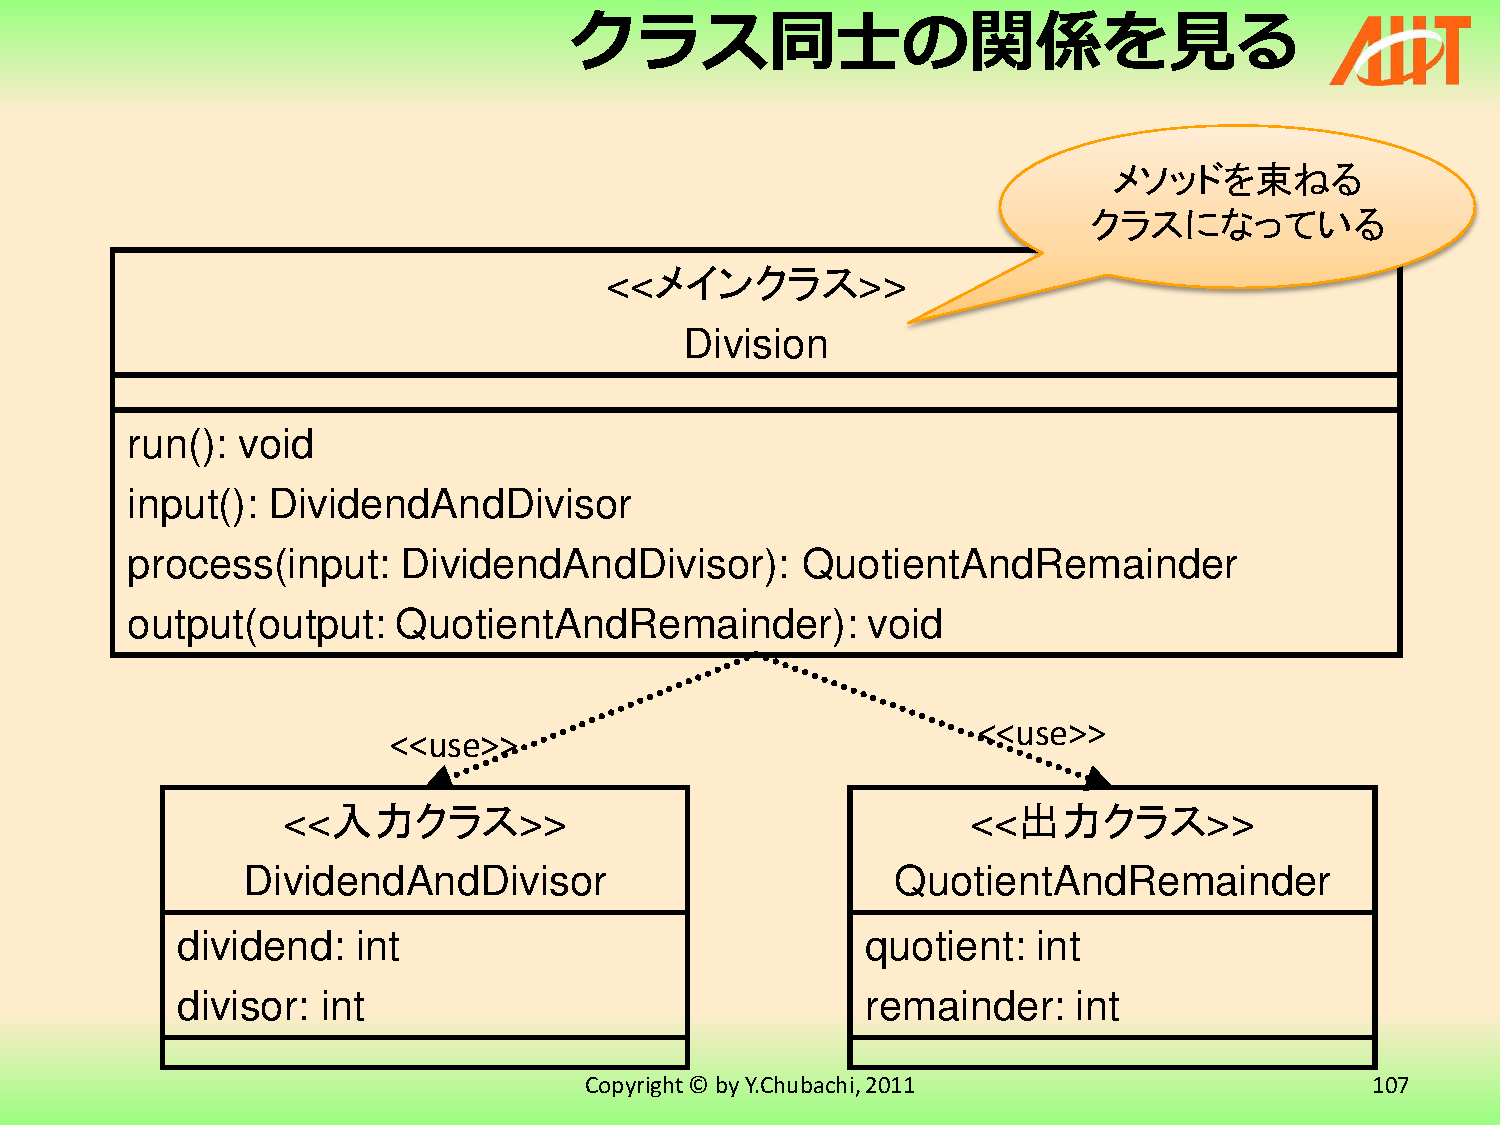
\includegraphics[width=0.8\textwidth, trim=15mm 0mm 15mm 0mm,clip]
   {Division.pdf}
  \caption{クラス同士の関係}
 \end{center}
\end{figure}

クラスの性質のここまでのまとめ

クラスの性質

 複数の情報(値)を束ねる
 ばらばらになっていた複数の入力値/出力値を束ねて,1つ
のまとまりとして取り扱う

 複数の処理を束ねる
 複数の関連する処理を束ねて,1つのまとまりとして取り
扱う

複数のクラス

 オブジェクト指向では,ネットワーク構造を備える
複数のクラスの関係により,アーキテクチャを構成
する

\section{2つのプログラムの共通構造を考える}
2つの目的の異なるプログラムをとりあげた

 「自乗を計算する」プログラム

 「割り算を計算する」プログラム

この両者のrun()を見比べて,何か気がつかない
だろうか?

 2つの異なるプログラムに共通する構造があるとき,
そこに「有用な抽象化」の可能性がある

自乗を計算するプログラム

\begin{verbatim}
	public void run() throws Exception {
	    double input = input();
	    double output = process(input);
	    output(output);
	}
\end{verbatim}

割り算をするプログラム

\begin{verbatim}
	public void run() throws Exception {
	    DividendAndDivisor input = input ();
	    QuotientAndRemainder output = process(input);
	    output (output);
	}
\end{verbatim}

両者は大同小異といえる.

同じ構造を再利用する

オブジェクト指向の特徴として「再利用性」が
ある

 目的の異なる2つのプログラムに共通する部分があ
れば,その部分を抽象化することで再利用可能

クラスとは,プログラムを再利用するための強
力な道具立てである

\begin{figure}
 \begin{center}
  %trim option's parameter order: left bottom right top
  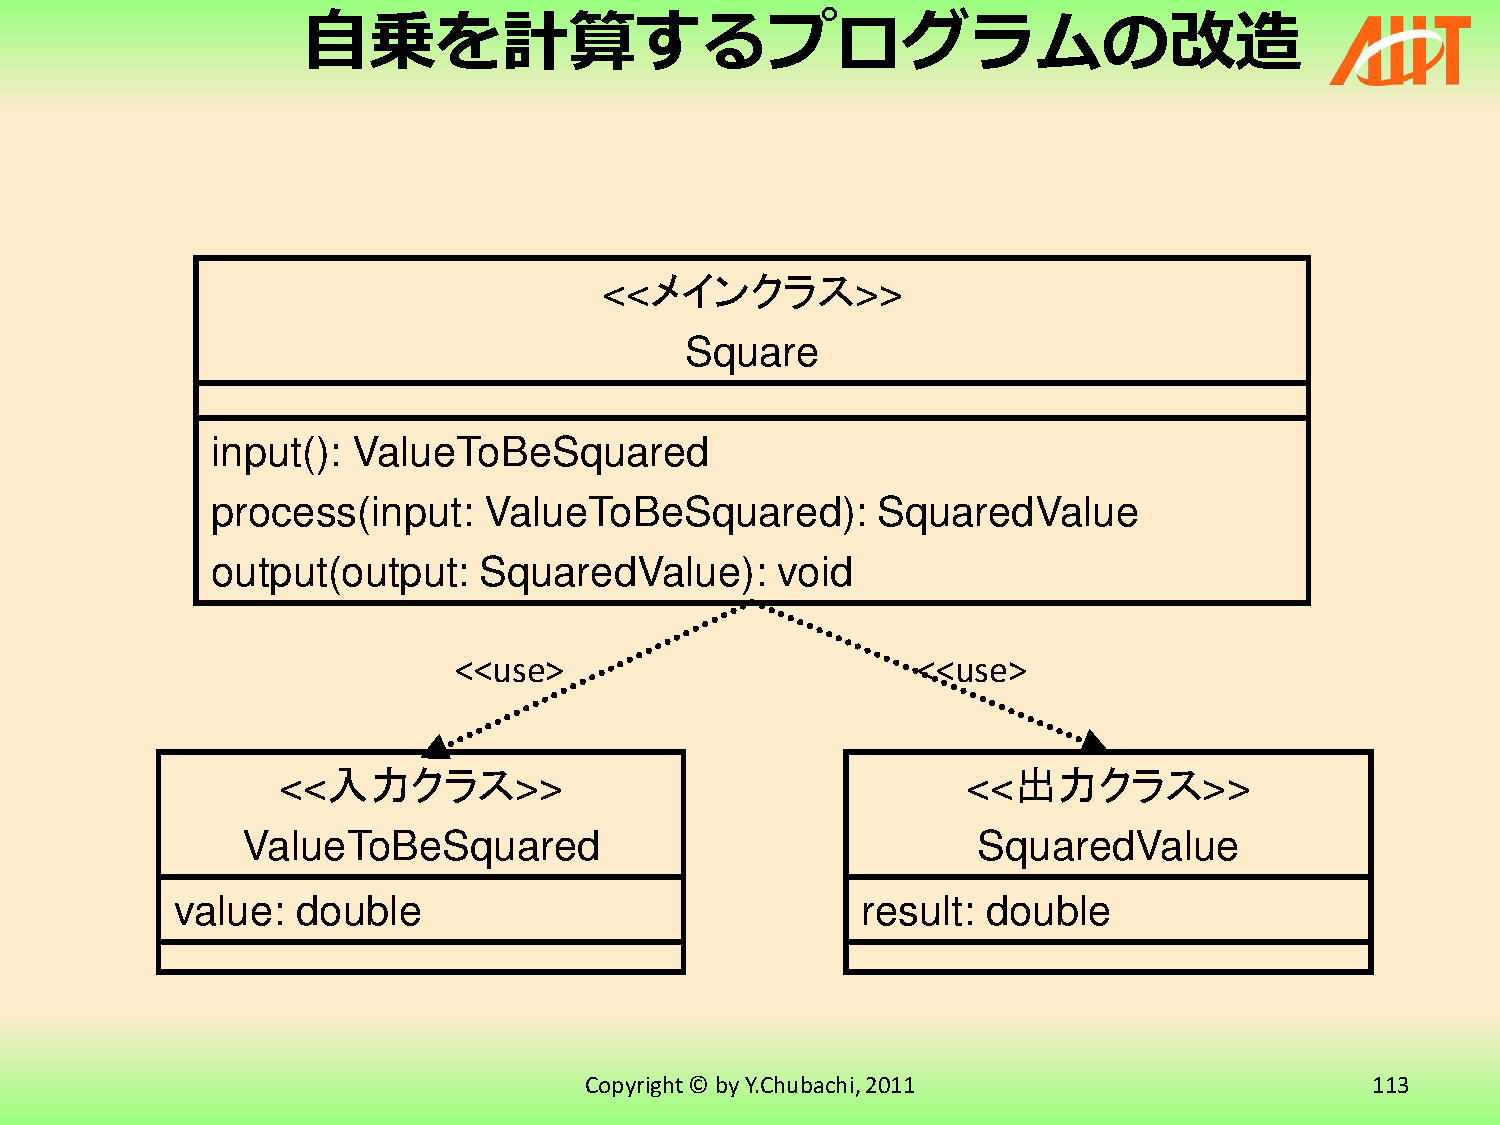
\includegraphics[width=0.8\textwidth, trim=15mm 0mm 15mm 0mm,clip]
   {Square.pdf}
  \caption{自乗を計算するプログラム}
 \end{center}
\end{figure}

\section{2つのプログラムの構造比較}

\begin{figure}
 \begin{center}
  %trim option's parameter order: left bottom right top
  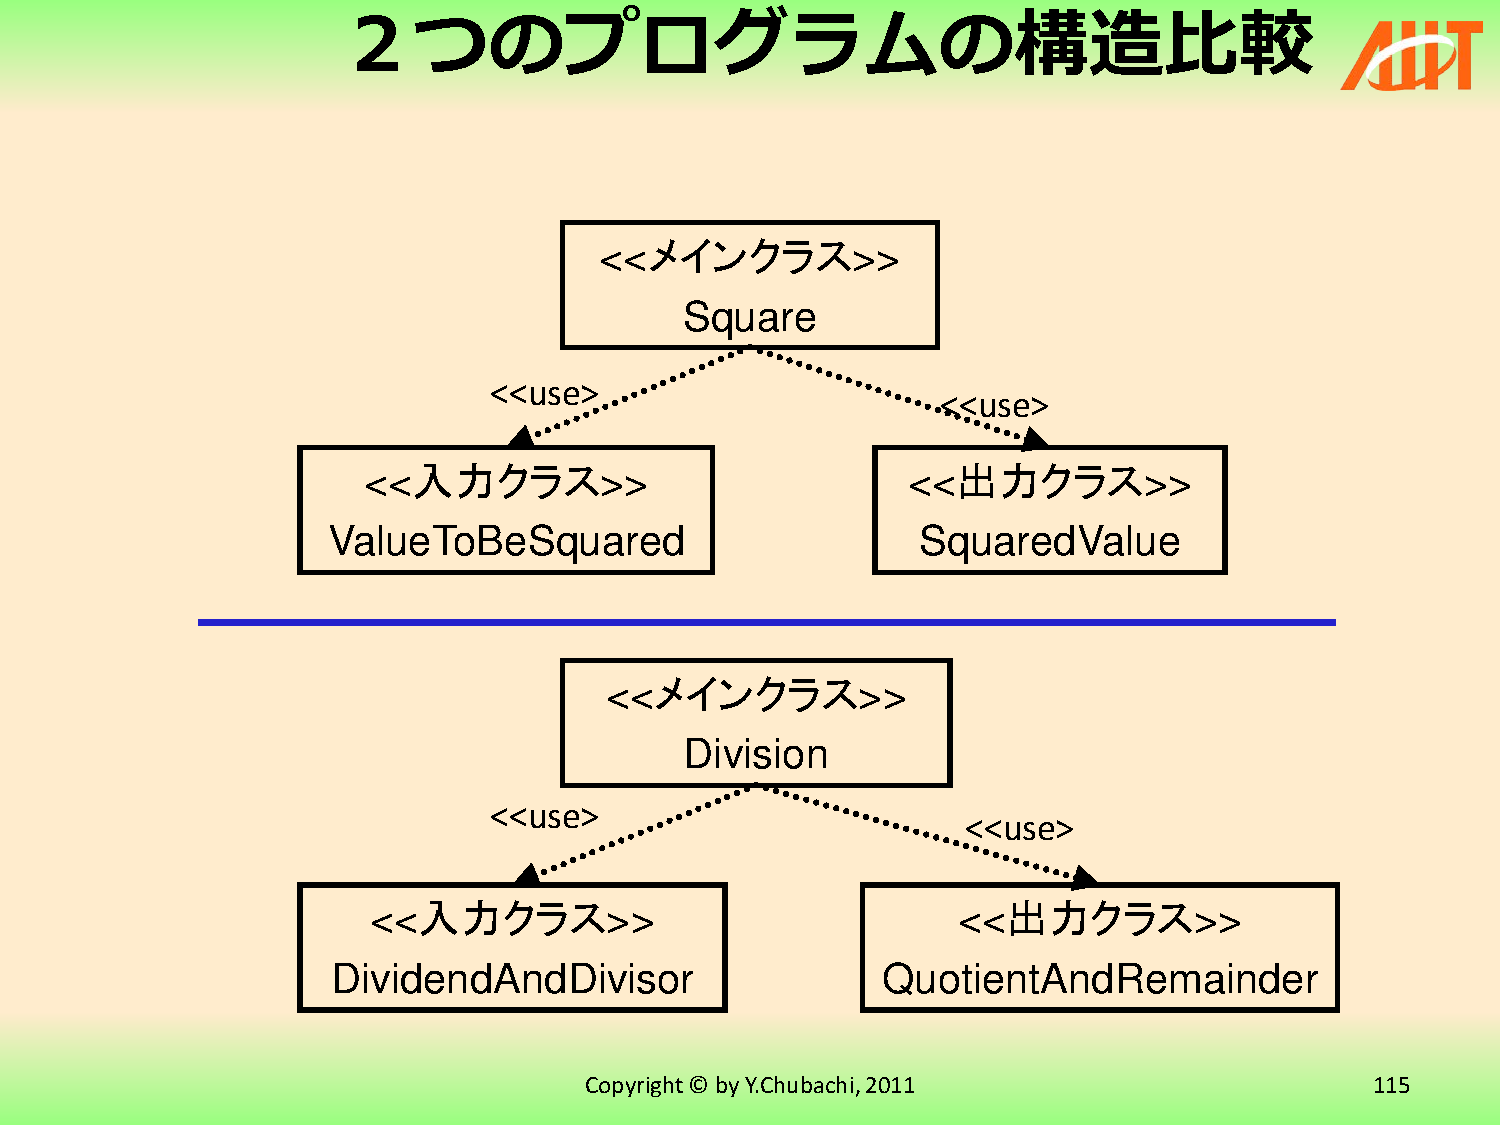
\includegraphics[width=0.8\textwidth, trim=15mm 0mm 15mm 0mm,clip]
   {Compare.pdf}
  \caption{構造比較}
 \end{center}
\end{figure}

\begin{figure}
 \begin{center}
  %trim option's parameter order: left bottom right top
  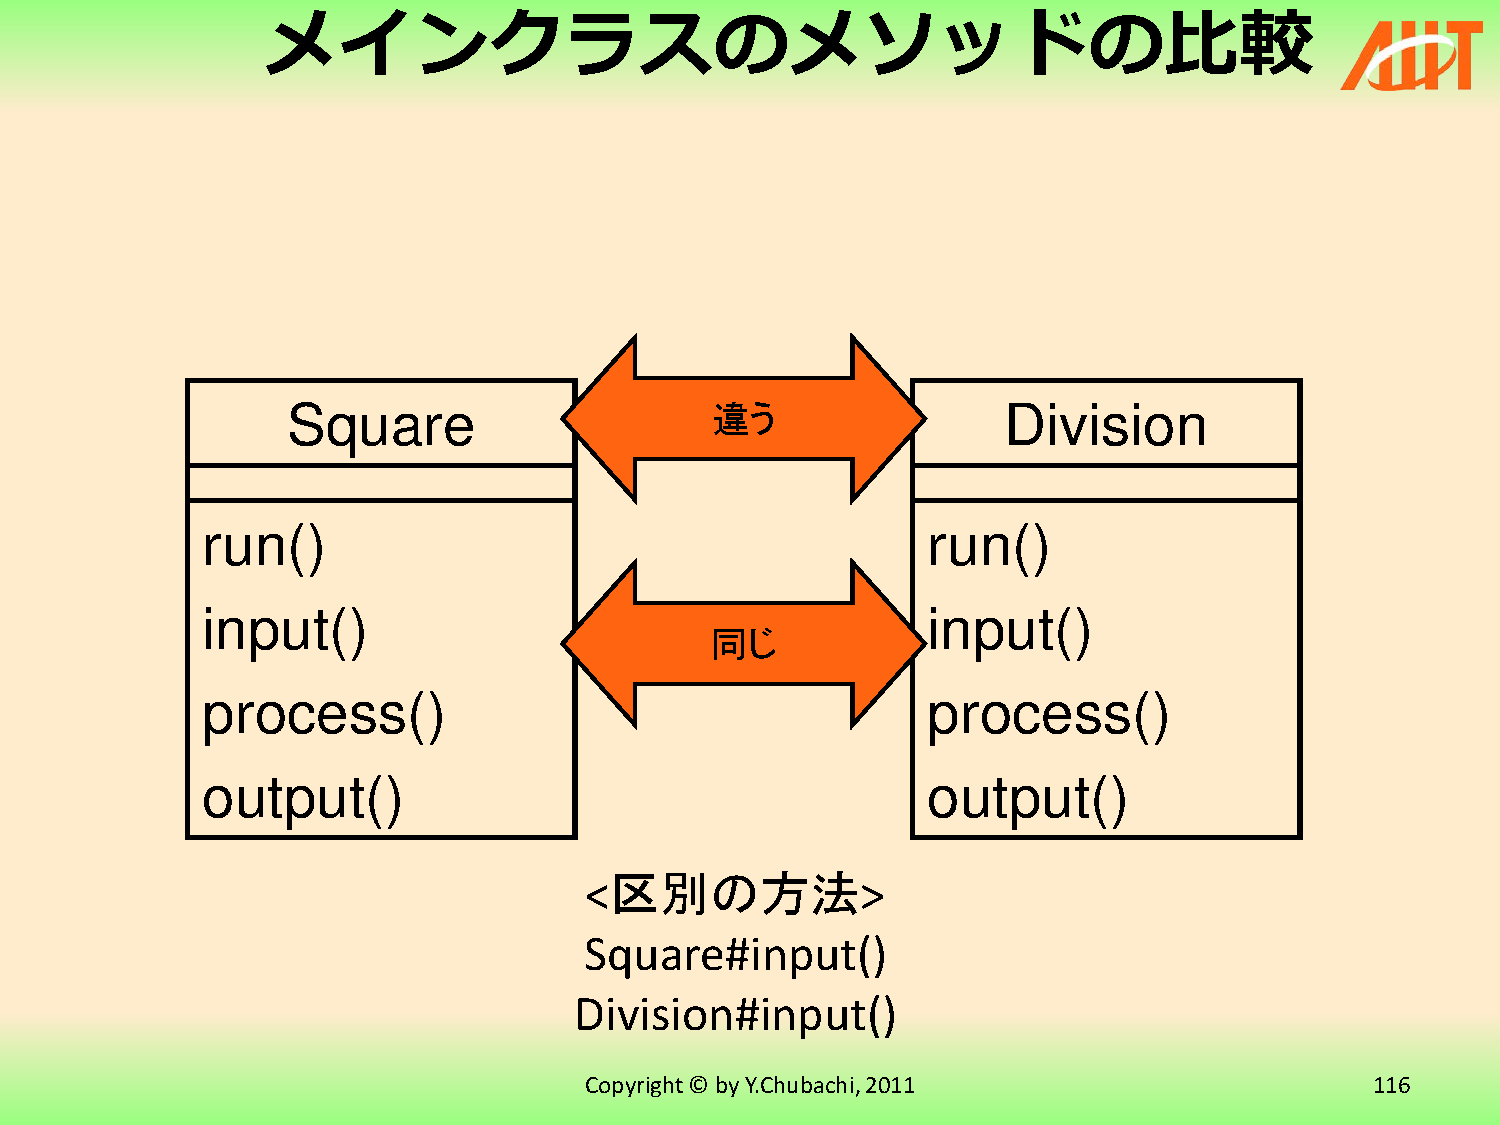
\includegraphics[width=0.8\textwidth, trim=15mm 0mm 15mm 0mm,clip]
   {CompareMethod.pdf}
  \caption{メインクラスのメソッドの比較}
 \end{center}
\end{figure}

\section{構造を共通にするには}
「自乗を計算する」プログラムと「割り算をする」プロ
グラムの入出力値をクラスにすることで,両者の構造が
「ほぼ」同一であることが明確になった.
「ほぼ」同一の構造は,オブジェクト指向の抽象化によ
り,「まったく同一」のプログラムにすることができる

やりたいこと

2つのプログラムの「run()」関数の中身を完全
に同じ記述にする

その上で,「run()」関数の中身を両方のプログ
ラムから再利用する

 最終的には,2つのプログラムの全てのクラスを同
じプロジェクトに入れて,双方のプログラムが同じ
メソッドを利用するようにする

ただし、最初はrun()の中身を同じにすることを
目指す

 同じコードが2箇所にある、という意味ではまだ再
利用とはいえないが、途中の過程として

「同じにする」ための議論
前のスライドを参考に,両方のrun()の中身を同
じにするにはどうしたらよいか,順を追って検
討してみよう

 入力値クラスと出力値クラス
 入力値変数と出力値変数
 入力メソッド,処理メソッド,出力メソッド

\section{インタフェイスを使ったアプローチ}

大同小異である二つのメソッドを,完全に同じものにす
るために,インタフェイスを使う方法がある.その方法
についてみていこう.

入出力値クラスについて
安直な解決方法
 両方のクラスを同じ名前にする
それがだめな理由
 プログラムにおいて,異なる概念を扱うクラスを同
じ名前にすることは好ましくない
 異なる概念を同じ名前にして扱うのは混乱のもと
 同じディレクトリ内に同一のファイル名を持つファイルが
作れないことと同様
– 「パッケージ」を分ける方法もあるが,ここでは考えない
よって,別な方法を考える

インタフェイスとは?
インタフェイスとは?

 メソッドのシグネチャのみを定義するクラスの一種
抽象クラスとの違い
 抽象クラスは,一部のメソッドの実装がない(=シグネ
チャのみの)クラス
インタフェイスVS抽象クラス
 シグネチャのみを記述するインタフェイスは,抽象クラス
よりも「軽量」である
 この性質は,分散オブジェクトの実現などに使われます
 あるクラスを継承させることを強要するより,インタフェ
イスを実装させることのほうが,影響度が少ない
「空っぽのインタフェイス」の存在意義
 シグネチャすらないインタフェイスは,あるものが他のも
のと同じ性質を備えることを示す「印」として利用可能

入力値クラスの共通化
インタフェイスを使った解決方法
 同じインタフェイスで「しるし」をつける


\begin{figure}
 \begin{center}
  %trim option's parameter order: left bottom right top
  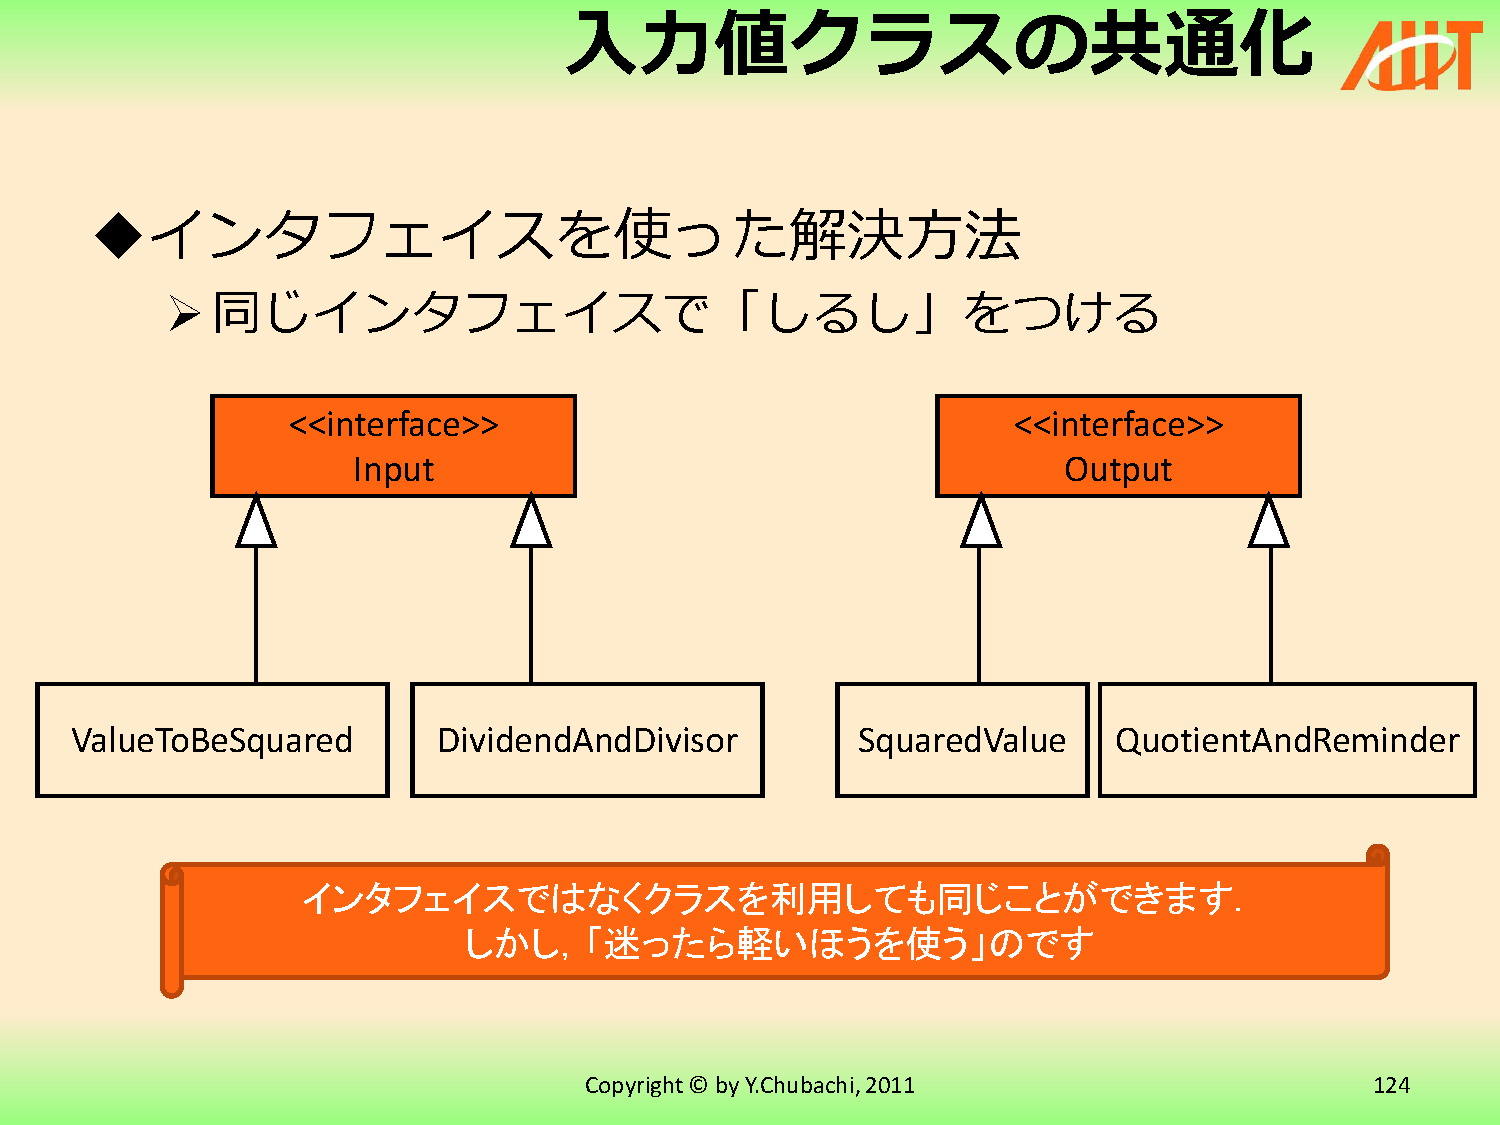
\includegraphics[width=0.8\textwidth, trim=15mm 0mm 15mm 0mm,clip]
   {Interface.pdf}
  \caption{インタフェイスの導入}
 \end{center}
\end{figure}

入出力用Interface

入力と出力のInterfaceのコード

Interfaceを実装させたコード

共通するrun()とメソッドのシグネチャ
pp.126

\section{差異を比較し上位概念を抽出}

2つのプログラムをまとめて,1つのプロジェクトとなった
いよいよ,同一の構造を再利用する形に変更していこう
そのためには,2つのプログラムの中心的なクラス(それらをメ
インクラスと呼ぼう)の上位概念を考える必要がある

異なる2つの上位にある概念」は何か?
2つのメイン・クラスの上位概念を表現するに
はどうしたらよいか?
この議論も,両者の現在の姿を比較することよ
り,共通部分と非共通部分を抽出することから
はじめよう

run()メソッド

 まったく同一である

IPOメソッド

 共通点

 メソッドのシグネチャ

 非共通点
 メソッドの中身

main() の共通点

共通化できそうな気配があるが・・・
後で議論!

\section{上位概念としてのFrameworkクラス}

自乗を計算するプログラムと,割り算を計算するプログ
ラムとで共通する部分を含む上位概念である,
Frameworkクラスを導入する

SquareとDivisionの上位概念
両者の共通部分を備える上位概念をクラスにする.

Frameworkには何を入れるべきか?
run()メソッド
 完全に共通するrun()をFrameworkに移すことには
異論がないだろう
IPOメソッドのシグネチャ
 run()が呼び出すIPOメソッドについては,中身は非
共通であるが,シグネチャは共通である
main()メソッド
 フレームワークの実態がSquareのインスタンスなの
かDivisionのインスタンスなのかを設定する部分であ
り,共通化できない
 実は,共通化は可能なのであるが,工夫が必要であるため
後回し

Frameworkはどんなクラスか?
(インスタンス化できる通常の)
クラスなのか?
・・・×

 FrawemorkはSquareかDivisionと必ず組み合わせて使う
必要があり,単体では成立しない
インタフェイスなのか?
・・・×

 メソッドのシグネチャだけであれば,それでもよいが,
run()の中身も持たせるため,インタフェイスではない
抽象クラスなのか?
・・・○

 run()メソッド(中身を含む)とIPOメソッド(シグネ
チャのみ)を備える抽象クラスとするのがよい

\begin{figure}
 \begin{center}
  %trim option's parameter order: left bottom right top
  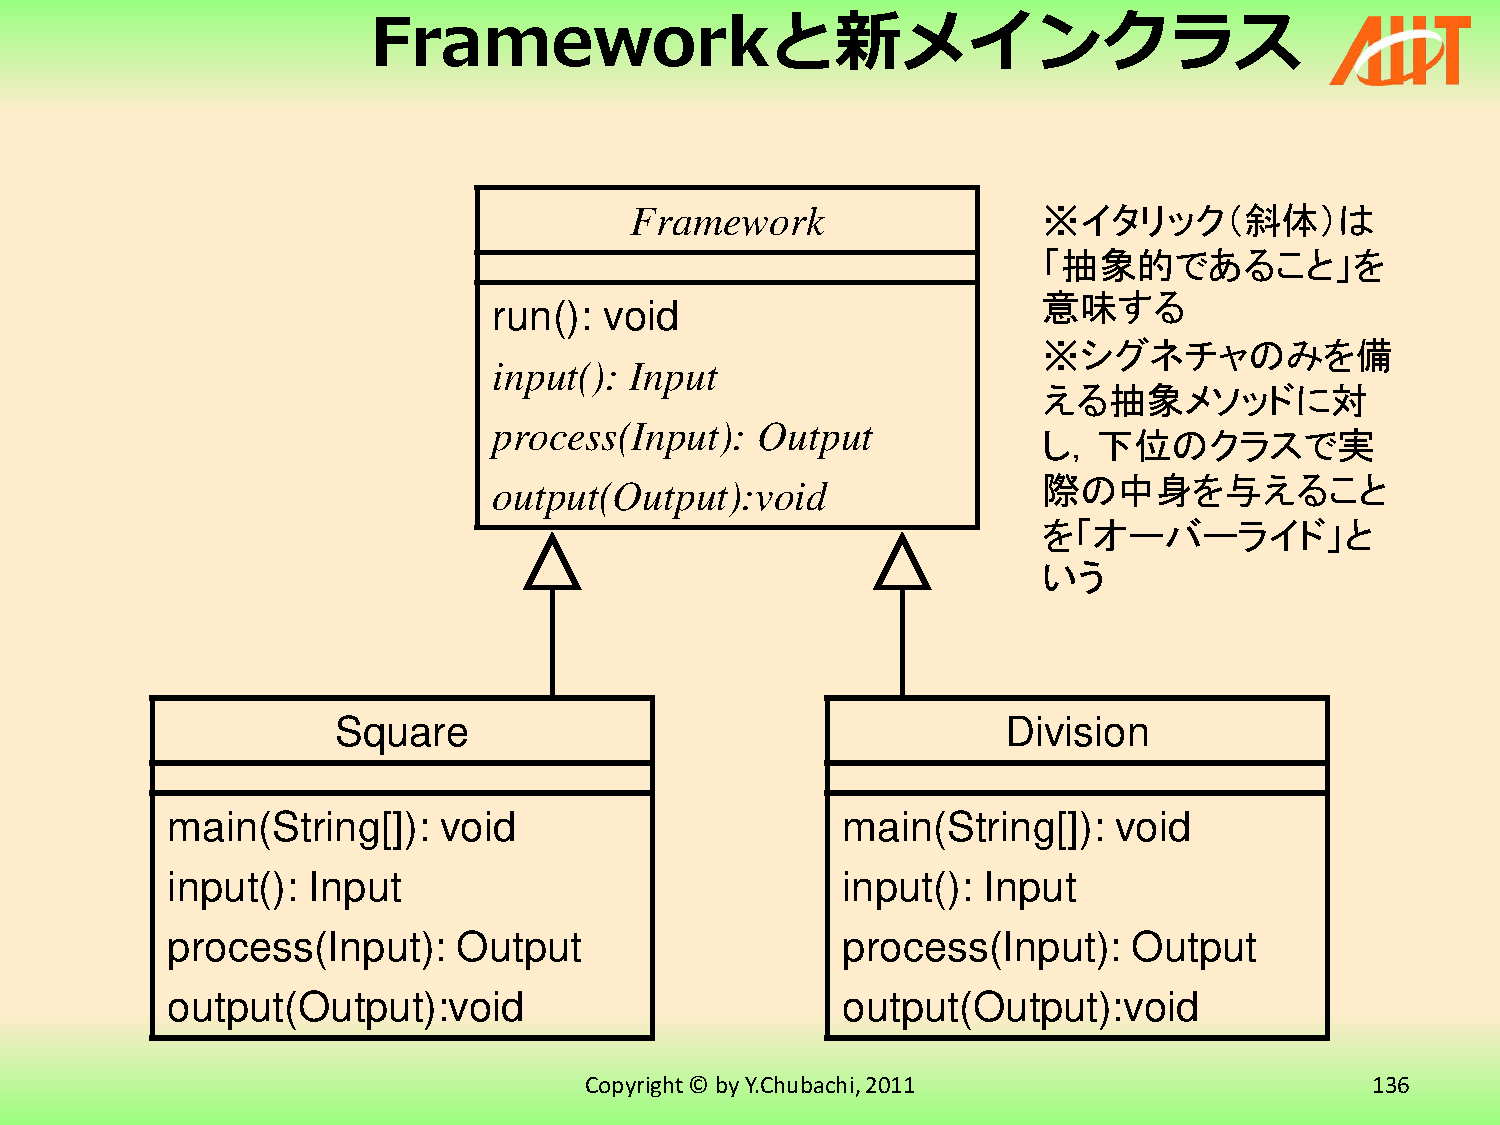
\includegraphics[width=0.8\textwidth, trim=15mm 0mm 15mm 0mm,clip]
   {FrameworkClass.pdf}
  \caption{Frameworkと新メインクラス}
 \end{center}
\end{figure}

修飾子(可視性)の変更
現在,main()以外のrun(),IPOメソッドの修飾
子はprivateである
 privateのメソッド(およびフィールド)は,他のク
ラスから完全に隠蔽される
 このままでは,下位クラスから呼び出したり,オー
バーライドしたりすることができない
修飾子をprotectedにすると解決
 protectedのメソッド(およびフィールド)は,それ
を継承する下位のクラスに対しては公開される

\section{pp.138--}

\newpage

\section{例題}
\subsection{Division4: フレームワーク化}


\subsection{Division5: }

\begin{figure}
 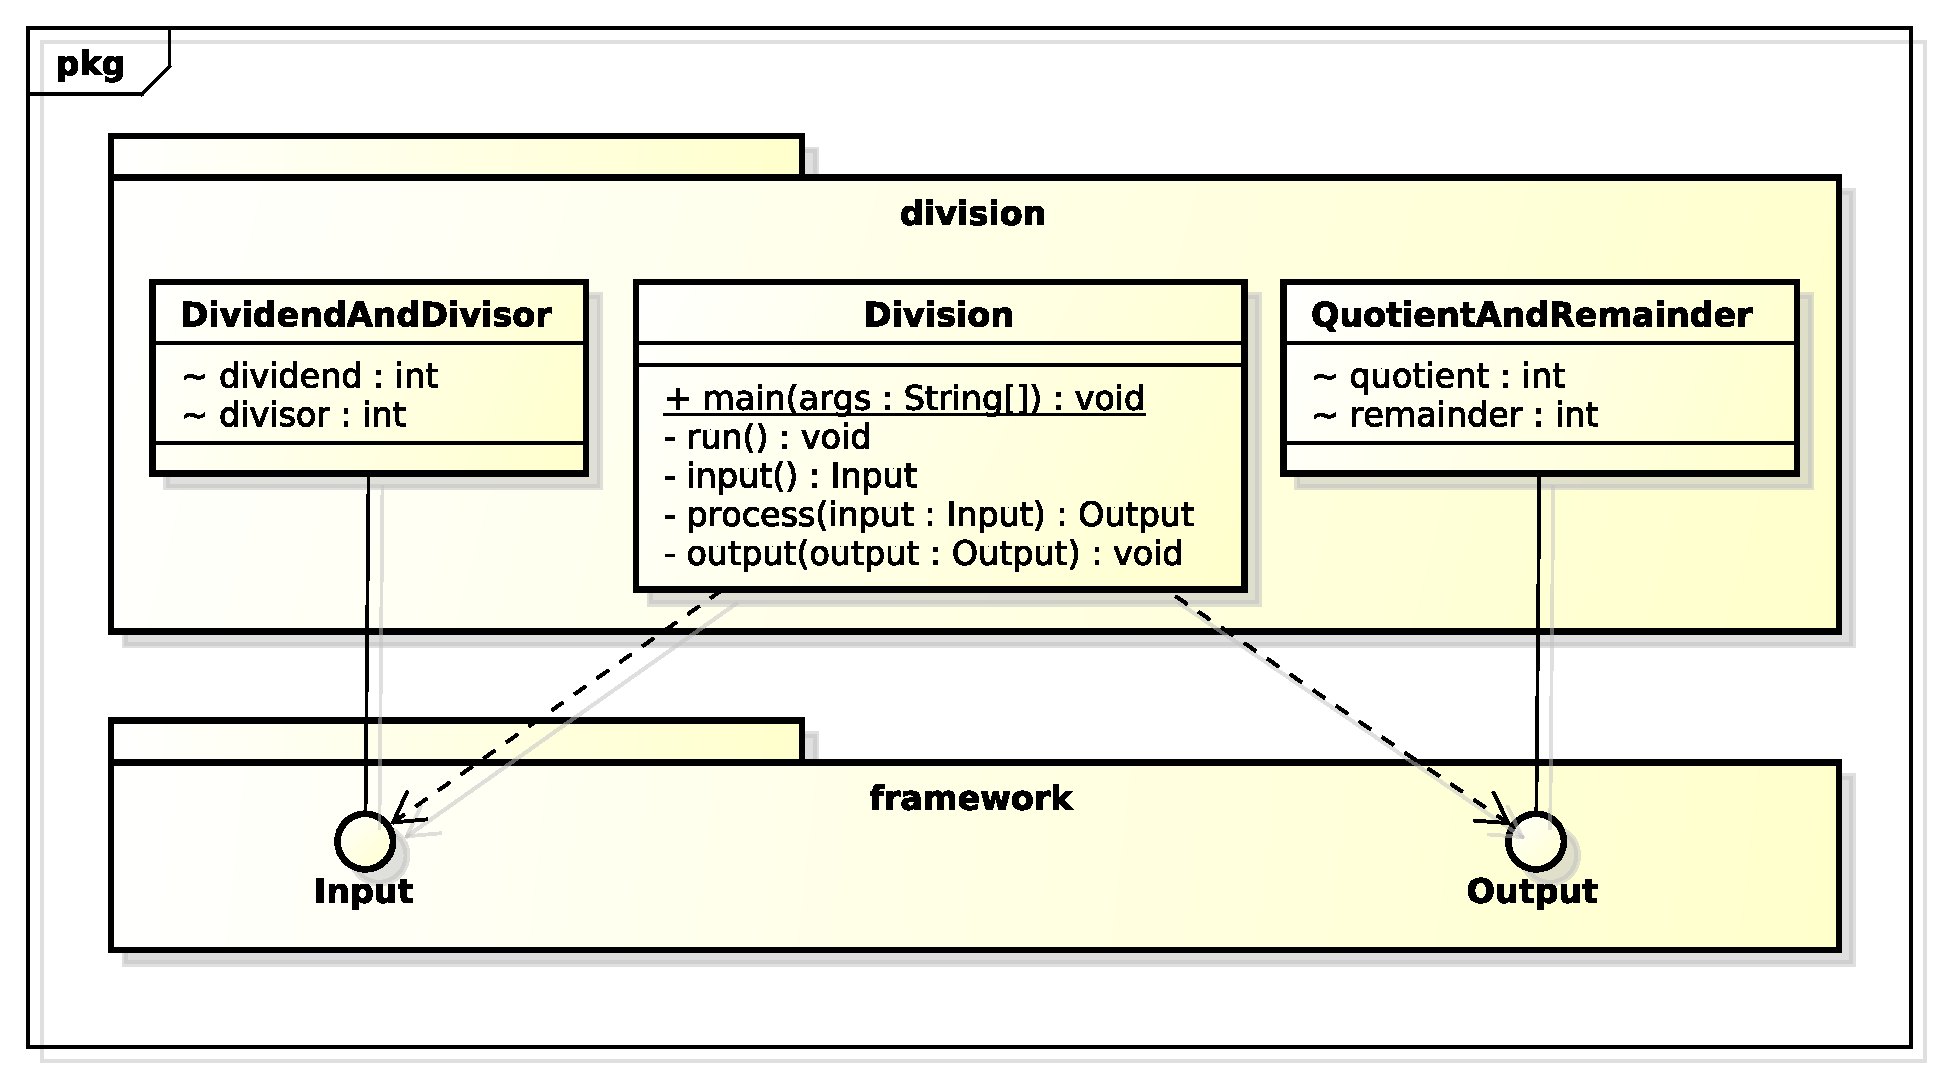
\includegraphics[width=\textwidth]{figures/Division5.pdf}
 \caption{Class diagram of Division5}
\end{figure}

frameworkパッケージがdivisionを支えている.まだまだへなちょこなフレームワークである.

\begin{figure}
 \begin{Verbatim}[commandchars=\\\{\},numbers=left,firstnumber=1,stepnumber=1,frame=single,fontsize=\small]
\PY{k+kn}{package}\PY{+w}{ }\PY{n}{division}\PY{o}{;}
\PY{k+kn}{import}\PY{+w}{ }\PY{n+nn}{java.io.BufferedReader}\PY{o}{;}
\PY{k+kn}{import}\PY{+w}{ }\PY{n+nn}{java.io.IOException}\PY{o}{;}
\PY{k+kn}{import}\PY{+w}{ }\PY{n+nn}{java.io.InputStreamReader}\PY{o}{;}

\PY{k+kn}{import}\PY{+w}{ }\PY{n+nn}{framework.Input}\PY{o}{;}
\PY{k+kn}{import}\PY{+w}{ }\PY{n+nn}{framework.Output}\PY{o}{;}


\PY{k+kd}{public}\PY{+w}{ }\PY{k+kd}{class}\PY{+w}{ }\PY{n+nc}{Division}\PY{+w}{ }\PY{o}{\PYZob{}}
\PY{+w}{    }\PY{k+kd}{public}\PY{+w}{ }\PY{k+kd}{static}\PY{+w}{ }\PY{k+kt}{void}\PY{+w}{ }\PY{n+nf}{main}\PY{o}{(}\PY{n}{String}\PY{o}{[}\PY{o}{]}\PY{+w}{ }\PY{n}{args}\PY{o}{)}\PY{+w}{ }\PY{k+kd}{throws}\PY{+w}{ }\PY{n}{Exception}\PY{+w}{ }\PY{o}{\PYZob{}}
\PY{+w}{    }\PY{+w}{    }\PY{n}{Division}\PY{+w}{ }\PY{n}{division}\PY{+w}{ }\PY{o}{=}\PY{+w}{ }\PY{k}{new}\PY{+w}{ }\PY{n}{Division}\PY{o}{(}\PY{o}{)}\PY{o}{;}
\PY{+w}{    }\PY{+w}{    }\PY{n}{division}\PY{o}{.}\PY{n+na}{run}\PY{o}{(}\PY{o}{)}\PY{o}{;}
\PY{+w}{    }\PY{o}{\PYZcb{}}
\PY{+w}{    }
\PY{+w}{    }
\PY{+w}{    }\PY{k+kd}{private}\PY{+w}{ }\PY{k+kt}{void}\PY{+w}{ }\PY{n+nf}{run}\PY{o}{(}\PY{o}{)}\PY{+w}{ }\PY{k+kd}{throws}\PY{+w}{ }\PY{n}{Exception}\PY{+w}{ }\PY{o}{\PYZob{}}
\PY{+w}{    }\PY{+w}{    }\PY{n}{Input}\PY{+w}{ }\PY{n}{input}\PY{+w}{ }\PY{o}{=}\PY{+w}{ }\PY{n}{input}\PY{o}{(}\PY{o}{)}\PY{o}{;}
\PY{+w}{    }\PY{+w}{    }\PY{n}{Output}\PY{+w}{ }\PY{n}{output}\PY{+w}{ }\PY{o}{=}\PY{+w}{ }\PY{n}{process}\PY{o}{(}\PY{n}{input}\PY{o}{)}\PY{o}{;}
\PY{+w}{    }\PY{+w}{    }\PY{n}{output}\PY{o}{(}\PY{n}{output}\PY{o}{)}\PY{o}{;}
\PY{+w}{    }\PY{o}{\PYZcb{}}

\PY{+w}{    }\PY{c+c1}{//}\PY{+w}{ }\PY{c+c1}{割られる数と割る数を読み込む}
\PY{+w}{    }\PY{k+kd}{private}\PY{+w}{ }\PY{n}{Input}\PY{+w}{ }\PY{n+nf}{input}\PY{o}{(}\PY{o}{)}\PY{+w}{ }\PY{k+kd}{throws}\PY{+w}{ }\PY{n}{IOException}\PY{+w}{ }\PY{o}{\PYZob{}}
\PY{+w}{    }\PY{+w}{    }\PY{n}{DividendAndDivisor}\PY{+w}{ }\PY{n}{input}\PY{+w}{ }\PY{o}{=}\PY{+w}{ }\PY{k}{new}\PY{+w}{ }\PY{n}{DividendAndDivisor}\PY{o}{(}\PY{o}{)}\PY{o}{;}
\PY{+w}{    }\PY{+w}{    }\PY{n}{BufferedReader}\PY{+w}{ }\PY{n}{reader}\PY{+w}{ }\PY{o}{=}
\PY{+w}{    }\PY{+w}{    }\PY{+w}{    }\PY{k}{new}\PY{+w}{ }\PY{n+nf}{BufferedReader}\PY{o}{(}\PY{k}{new}\PY{+w}{ }\PY{n}{InputStreamReader}\PY{o}{(}\PY{n}{System}\PY{o}{.}\PY{n+na}{in}\PY{o}{)}\PY{o}{)}\PY{o}{;}
\PY{+w}{    }\PY{+w}{    }\PY{n}{System}\PY{o}{.}\PY{n+na}{out}\PY{o}{.}\PY{n+na}{print}\PY{o}{(}\PY{l+s}{"割られる数を入力してください:"}\PY{o}{)}\PY{o}{;}
\PY{+w}{    }\PY{+w}{    }\PY{n}{String}\PY{+w}{ }\PY{n}{dividendString}\PY{+w}{ }\PY{o}{=}\PY{+w}{ }\PY{n}{reader}\PY{o}{.}\PY{n+na}{readLine}\PY{o}{(}\PY{o}{)}\PY{o}{;}
\PY{+w}{    }\PY{+w}{    }\PY{n}{input}\PY{o}{.}\PY{n+na}{dividend}\PY{+w}{ }\PY{o}{=}\PY{+w}{ }\PY{n}{Integer}\PY{o}{.}\PY{n+na}{parseInt}\PY{o}{(}\PY{n}{dividendString}\PY{o}{)}\PY{o}{;}
\PY{+w}{    }\PY{+w}{    }\PY{n}{System}\PY{o}{.}\PY{n+na}{out}\PY{o}{.}\PY{n+na}{print}\PY{o}{(}\PY{l+s}{"割る数を入力してください:"}\PY{o}{)}\PY{o}{;}
\PY{+w}{    }\PY{+w}{    }\PY{n}{String}\PY{+w}{ }\PY{n}{divisorString}\PY{+w}{ }\PY{o}{=}\PY{+w}{ }\PY{n}{reader}\PY{o}{.}\PY{n+na}{readLine}\PY{o}{(}\PY{o}{)}\PY{o}{;}
\PY{+w}{    }\PY{+w}{    }\PY{n}{input}\PY{o}{.}\PY{n+na}{divisor}\PY{+w}{ }\PY{o}{=}\PY{+w}{ }\PY{n}{Integer}\PY{o}{.}\PY{n+na}{parseInt}\PY{o}{(}\PY{n}{divisorString}\PY{o}{)}\PY{o}{;}
\PY{+w}{    }\PY{+w}{    }\PY{k}{return}\PY{+w}{ }\PY{n}{input}\PY{o}{;}
\PY{+w}{    }\PY{o}{\PYZcb{}}

\PY{+w}{    }\PY{c+c1}{//}\PY{+w}{ }\PY{c+c1}{商と余を計算する}
\PY{+w}{    }\PY{k+kd}{private}\PY{+w}{ }\PY{n}{Output}\PY{+w}{ }\PY{n+nf}{process}\PY{o}{(}\PY{n}{Input}\PY{+w}{ }\PY{n}{input}\PY{o}{)}\PY{+w}{ }\PY{o}{\PYZob{}}
\PY{+w}{    }\PY{+w}{    }\PY{n}{DividendAndDivisor}\PY{+w}{ }\PY{n}{dad}\PY{+w}{ }\PY{o}{=}\PY{+w}{ }\PY{o}{(}\PY{n}{DividendAndDivisor}\PY{o}{)}\PY{+w}{ }\PY{n}{input}\PY{o}{;}
\PY{+w}{    }\PY{+w}{    }\PY{n}{QuotientAndRemainder}\PY{+w}{ }\PY{n}{output}\PY{+w}{ }\PY{o}{=}\PY{+w}{ }\PY{k}{new}\PY{+w}{ }\PY{n}{QuotientAndRemainder}\PY{o}{(}\PY{o}{)}\PY{o}{;}
\PY{+w}{    }\PY{+w}{    }\PY{n}{output}\PY{o}{.}\PY{n+na}{quotient}\PY{+w}{ }\PY{o}{=}\PY{+w}{ }\PY{n}{dad}\PY{o}{.}\PY{n+na}{dividend}\PY{+w}{ }\PY{o}{/}\PY{+w}{ }\PY{n}{dad}\PY{o}{.}\PY{n+na}{divisor}\PY{o}{;}
\PY{+w}{    }\PY{+w}{    }\PY{n}{output}\PY{o}{.}\PY{n+na}{remainder}\PY{+w}{ }\PY{o}{=}\PY{+w}{ }\PY{n}{dad}\PY{o}{.}\PY{n+na}{dividend}\PY{+w}{ }\PY{o}{\PYZpc{}}\PY{+w}{ }\PY{n}{dad}\PY{o}{.}\PY{n+na}{divisor}\PY{o}{;}
\PY{+w}{    }\PY{+w}{    }\PY{k}{return}\PY{+w}{ }\PY{n}{output}\PY{o}{;}
\PY{+w}{    }\PY{o}{\PYZcb{}}

\PY{+w}{    }\PY{c+c1}{//}\PY{+w}{ }\PY{c+c1}{割り算の結果を表示する}
\PY{+w}{    }\PY{k+kd}{private}\PY{+w}{ }\PY{k+kt}{void}\PY{+w}{ }\PY{n+nf}{output}\PY{o}{(}\PY{n}{Output}\PY{+w}{ }\PY{n}{output}\PY{o}{)}\PY{+w}{ }\PY{o}{\PYZob{}}
\PY{+w}{    }\PY{+w}{    }\PY{n}{QuotientAndRemainder}\PY{+w}{ }\PY{n}{qar}\PY{+w}{ }\PY{o}{=}\PY{+w}{ }\PY{o}{(}\PY{n}{QuotientAndRemainder}\PY{o}{)}\PY{+w}{ }\PY{n}{output}\PY{o}{;}
\PY{+w}{    }\PY{+w}{    }\PY{n}{System}\PY{o}{.}\PY{n+na}{out}\PY{o}{.}\PY{n+na}{print}\PY{o}{(}\PY{l+s}{"商は"}\PY{+w}{ }\PY{o}{+}\PY{+w}{ }\PY{n}{qar}\PY{o}{.}\PY{n+na}{quotient}\PY{+w}{ }\PY{o}{+}\PY{+w}{ }\PY{l+s}{"で余は"}\PY{+w}{ }\PY{o}{+}\PY{+w}{ }\PY{n}{qar}\PY{o}{.}\PY{n+na}{remainder}\PY{+w}{ }\PY{o}{+}\PY{+w}{ }\PY{l+s}{"です"}\PY{o}{)}\PY{o}{;}
\PY{+w}{    }\PY{o}{\PYZcb{}}
\PY{o}{\PYZcb{}}
\end{Verbatim}

 \caption{Division5: }
\end{figure}

\section{演習}
\subsection{Square5: 「枠(わく)」を抽出する}

frameworkパッケージには次の2つのインタフェイスを抽出しよう.

\begin{Verbatim}[commandchars=\\\{\},numbers=left,firstnumber=1,stepnumber=1,frame=single,fontsize=\small]
\PY{k+kn}{package}\PY{+w}{ }\PY{n}{framework}\PY{o}{;}

\PY{k+kd}{public}\PY{+w}{ }\PY{k+kd}{interface}\PY{+w}{ }\PY{n+nc}{Input}\PY{+w}{ }\PY{o}{\PYZob{}}

\PY{o}{\PYZcb{}}
\end{Verbatim}

\begin{Verbatim}[commandchars=\\\{\},numbers=left,firstnumber=1,stepnumber=1,frame=single,fontsize=\small]
\PY{k+kn}{package}\PY{+w}{ }\PY{n}{framework}\PY{o}{;}

\PY{k+kd}{public}\PY{+w}{ }\PY{k+kd}{interface}\PY{+w}{ }\PY{n+nc}{Output}\PY{+w}{ }\PY{o}{\PYZob{}}

\PY{o}{\PYZcb{}}
\end{Verbatim}


すでにある入力値・出力値のクラスにそれぞれ,インタフェイスを実装する.

\begin{Verbatim}[commandchars=\\\{\},numbers=left,firstnumber=1,stepnumber=1,frame=single,fontsize=\small]
\PY{k+kn}{package}\PY{+w}{ }\PY{n}{square}\PY{o}{;}

\PY{k+kn}{import}\PY{+w}{ }\PY{n+nn}{framework.Input}\PY{o}{;}

\PY{k+kd}{class}\PY{+w}{ }\PY{n+nc}{ValueToBeSquared}\PY{+w}{ }\PY{k+kd}{implements}\PY{+w}{ }\PY{n}{Input}\PY{+w}{ }\PY{o}{\PYZob{}}
\PY{+w}{    }\PY{k+kt}{double}\PY{+w}{ }\PY{n}{value}\PY{o}{;}
\PY{o}{\PYZcb{}}
\end{Verbatim}

\begin{Verbatim}[commandchars=\\\{\},numbers=left,firstnumber=1,stepnumber=1,frame=single,fontsize=\small]
\PY{k+kn}{package}\PY{+w}{ }\PY{n}{square}\PY{o}{;}

\PY{k+kn}{import}\PY{+w}{ }\PY{n+nn}{framework.Output}\PY{o}{;}

\PY{k+kd}{class}\PY{+w}{ }\PY{n+nc}{SquaredValue}\PY{+w}{ }\PY{k+kd}{implements}\PY{+w}{ }\PY{n}{Output}\PY{+w}{ }\PY{o}{\PYZob{}}
\PY{+w}{    }\PY{k+kt}{double}\PY{+w}{ }\PY{n}{result}\PY{o}{;}
\PY{o}{\PYZcb{}}
\end{Verbatim}


\newpage
\begin{Verbatim}[commandchars=\\\{\},numbers=left,firstnumber=1,stepnumber=1,frame=single,fontsize=\small]
\PY{k+kn}{package}\PY{+w}{ }\PY{n}{square}\PY{o}{;}

\PY{k+kn}{import}\PY{+w}{ }\PY{n+nn}{java.io.BufferedReader}\PY{o}{;}
\PY{k+kn}{import}\PY{+w}{ }\PY{n+nn}{java.io.IOException}\PY{o}{;}
\PY{k+kn}{import}\PY{+w}{ }\PY{n+nn}{java.io.InputStreamReader}\PY{o}{;}

\PY{k+kn}{import}\PY{+w}{ }\PY{n+nn}{framework.Input}\PY{o}{;}
\PY{k+kn}{import}\PY{+w}{ }\PY{n+nn}{framework.Output}\PY{o}{;}

\PY{k+kd}{public}\PY{+w}{ }\PY{k+kd}{class}\PY{+w}{ }\PY{n+nc}{Square}\PY{+w}{ }\PY{o}{\PYZob{}}
\PY{+w}{    }\PY{k+kd}{public}\PY{+w}{ }\PY{k+kd}{static}\PY{+w}{ }\PY{k+kt}{void}\PY{+w}{ }\PY{n+nf}{main}\PY{o}{(}\PY{n}{String}\PY{o}{[}\PY{o}{]}\PY{+w}{ }\PY{n}{args}\PY{o}{)}\PY{+w}{ }\PY{k+kd}{throws}\PY{+w}{ }\PY{n}{Exception}\PY{+w}{ }\PY{o}{\PYZob{}}
\PY{+w}{    }\PY{+w}{    }\PY{n}{Square}\PY{+w}{ }\PY{n}{square}\PY{+w}{ }\PY{o}{=}\PY{+w}{ }\PY{k}{new}\PY{+w}{ }\PY{n}{Square}\PY{o}{(}\PY{o}{)}\PY{o}{;}
\PY{+w}{    }\PY{+w}{    }\PY{n}{square}\PY{o}{.}\PY{n+na}{run}\PY{o}{(}\PY{o}{)}\PY{o}{;}
\PY{+w}{    }\PY{o}{\PYZcb{}}

\PY{+w}{    }\PY{k+kd}{private}\PY{+w}{ }\PY{k+kt}{void}\PY{+w}{ }\PY{n+nf}{run}\PY{o}{(}\PY{o}{)}\PY{+w}{ }\PY{k+kd}{throws}\PY{+w}{ }\PY{n}{Exception}\PY{+w}{ }\PY{o}{\PYZob{}}
\PY{+w}{    }\PY{+w}{    }\PY{n}{Input}\PY{+w}{ }\PY{n}{input}\PY{+w}{ }\PY{o}{=}\PY{+w}{ }\PY{n}{input}\PY{o}{(}\PY{o}{)}\PY{o}{;}
\PY{+w}{    }\PY{+w}{    }\PY{n}{Output}\PY{+w}{ }\PY{n}{output}\PY{+w}{ }\PY{o}{=}\PY{+w}{ }\PY{n}{process}\PY{o}{(}\PY{n}{input}\PY{o}{)}\PY{o}{;}
\PY{+w}{    }\PY{+w}{    }\PY{n}{output}\PY{o}{(}\PY{n}{output}\PY{o}{)}\PY{o}{;}
\PY{+w}{    }\PY{o}{\PYZcb{}}

\PY{+w}{    }\PY{c+c1}{//}\PY{+w}{ }\PY{c+c1}{自乗を計算する値を入力する}
\PY{+w}{    }\PY{k+kd}{private}\PY{+w}{ }\PY{n}{Input}\PY{+w}{ }\PY{n+nf}{input}\PY{o}{(}\PY{o}{)}\PY{+w}{ }\PY{k+kd}{throws}\PY{+w}{ }\PY{n}{IOException}\PY{+w}{ }\PY{o}{\PYZob{}}
\PY{+w}{    }\PY{+w}{    }\PY{n}{ValueToBeSquared}\PY{+w}{ }\PY{n}{input}\PY{+w}{ }\PY{o}{=}\PY{+w}{ }\PY{k}{new}\PY{+w}{ }\PY{n}{ValueToBeSquared}\PY{o}{(}\PY{o}{)}\PY{o}{;}
\PY{+w}{    }\PY{+w}{    }\PY{n}{System}\PY{o}{.}\PY{n+na}{out}\PY{o}{.}\PY{n+na}{print}\PY{o}{(}\PY{l+s}{"自乗を計算する値を入力してください:"}\PY{o}{)}\PY{o}{;}
\PY{+w}{    }\PY{+w}{    }\PY{n}{BufferedReader}\PY{+w}{ }\PY{n}{reader}\PY{+w}{ }\PY{o}{=}
\PY{+w}{    }\PY{+w}{    }\PY{+w}{    }\PY{k}{new}\PY{+w}{ }\PY{n+nf}{BufferedReader}\PY{o}{(}
\PY{+w}{    }\PY{+w}{    }\PY{+w}{    }\PY{+w}{    }\PY{k}{new}\PY{+w}{ }\PY{n+nf}{InputStreamReader}\PY{o}{(}\PY{n}{System}\PY{o}{.}\PY{n+na}{in}\PY{o}{)}\PY{o}{)}\PY{o}{;}
\PY{+w}{    }\PY{+w}{    }\PY{n}{String}\PY{+w}{ }\PY{n}{valueString}\PY{+w}{ }\PY{o}{=}\PY{+w}{ }\PY{n}{reader}\PY{o}{.}\PY{n+na}{readLine}\PY{o}{(}\PY{o}{)}\PY{o}{;}
\PY{+w}{    }\PY{+w}{    }\PY{n}{input}\PY{o}{.}\PY{n+na}{value}\PY{+w}{ }\PY{o}{=}\PY{+w}{ }\PY{n}{Double}\PY{o}{.}\PY{n+na}{parseDouble}\PY{o}{(}\PY{n}{valueString}\PY{o}{)}\PY{o}{;}
\PY{+w}{    }\PY{+w}{    }\PY{k}{return}\PY{+w}{ }\PY{n}{input}\PY{o}{;}
\PY{+w}{    }\PY{o}{\PYZcb{}}

\PY{+w}{    }\PY{c+c1}{//}\PY{+w}{ }\PY{c+c1}{自乗を計算する}
\PY{+w}{    }\PY{k+kd}{private}\PY{+w}{ }\PY{n}{Output}\PY{+w}{ }\PY{n+nf}{process}\PY{o}{(}\PY{n}{Input}\PY{+w}{ }\PY{n}{input}\PY{o}{)}\PY{+w}{ }\PY{o}{\PYZob{}}
\PY{+w}{    }\PY{+w}{    }\PY{n}{ValueToBeSquared}\PY{+w}{ }\PY{n}{vtbs}\PY{+w}{ }\PY{o}{=}\PY{o}{(}\PY{n}{ValueToBeSquared}\PY{o}{)}\PY{+w}{ }\PY{n}{input}\PY{o}{;}
\PY{+w}{    }\PY{+w}{    }\PY{n}{SquaredValue}\PY{+w}{ }\PY{n}{output}\PY{+w}{ }\PY{o}{=}\PY{+w}{ }\PY{k}{new}\PY{+w}{ }\PY{n}{SquaredValue}\PY{o}{(}\PY{o}{)}\PY{o}{;}
\PY{+w}{    }\PY{+w}{    }\PY{n}{output}\PY{o}{.}\PY{n+na}{result}\PY{+w}{ }\PY{o}{=}\PY{+w}{ }\PY{n}{vtbs}\PY{o}{.}\PY{n+na}{value}\PY{+w}{ }\PY{o}{*}\PY{+w}{ }\PY{n}{vtbs}\PY{o}{.}\PY{n+na}{value}\PY{o}{;}
\PY{+w}{    }\PY{+w}{    }\PY{k}{return}\PY{+w}{ }\PY{n}{output}\PY{o}{;}
\PY{+w}{    }\PY{o}{\PYZcb{}}

\PY{+w}{    }\PY{c+c1}{//}\PY{+w}{ }\PY{c+c1}{計算結果を出力する}
\PY{+w}{    }\PY{k+kd}{private}\PY{+w}{ }\PY{k+kt}{void}\PY{+w}{ }\PY{n+nf}{output}\PY{o}{(}\PY{n}{Output}\PY{+w}{ }\PY{n}{output}\PY{o}{)}\PY{+w}{ }\PY{o}{\PYZob{}}
\PY{+w}{    }\PY{+w}{    }\PY{n}{SquaredValue}\PY{+w}{ }\PY{n}{sv}\PY{+w}{ }\PY{o}{=}\PY{+w}{ }\PY{o}{(}\PY{n}{SquaredValue}\PY{o}{)}\PY{+w}{ }\PY{n}{output}\PY{o}{;}
\PY{+w}{    }\PY{+w}{    }\PY{n}{System}\PY{o}{.}\PY{n+na}{out}\PY{o}{.}\PY{n+na}{println}\PY{o}{(}\PY{l+s}{"計算結果:"}\PY{+w}{ }\PY{o}{+}\PY{+w}{ }\PY{n}{sv}\PY{o}{.}\PY{n+na}{result}\PY{o}{)}\PY{o}{;}
\PY{+w}{    }\PY{o}{\PYZcb{}}
\PY{o}{\PYZcb{}}
\end{Verbatim}

\newpage


\chapter{メモ}

\begin{enumerate}
 \item 名前付けと抽象化について(int x = 1; double pi = 3.14)
 \item テストを取り上げるか?
 \item パターンとアーキテクチャについて解説する?
 \item UMLの関連・依存関係について
 \item ライブコーディング
 \item 防衛的プログラミング
 \item interfaceとclassの使い分け
 \item 試行錯誤.あるべき設計を発見するまでに必要だったプロセスvs手
       戻り
 \item パッケージは名前空間です,という説明をどこかでする.
\end{enumerate}

Eclipseに関するスライドpp.74--89をどうするか.

オブジェクト指向は概念に基づく・・・.

オブジェクト指向における抽象化とは,情報と処理のカプセルを抽出して一位
に識別できる名前をつけること.

\begin{演習}
 Java言語ではクラスの名前とファイル名を一致させる必要がある.他のオブジェ
 クト指向型言語の場合を調べよ.また,クラス名とファイル名を一致させるこ
 との長所・短所について考察せよ.
\end{演習}
\end{document}
